\documentclass[aps,prc,twocolumn,superscriptaddress,floatfix]{revtex4-1}
\usepackage[english]{babel}
\usepackage[T1]{fontenc}
\usepackage[colorlinks=true,linkcolor=blue,citecolor=blue,urlcolor=blue]{hyperref}
\usepackage{bm,bbm,amssymb,amsmath}
\usepackage{graphicx}
\usepackage{multirow,booktabs}
\usepackage{isotope}
\usepackage{physics}
\usepackage[capitalize]{cleveref}
\newcommand{\crefrangeconjunction}{--}

\setlength{\tabcolsep}{10pt}
\newcommand{\red}[1]{\protect\textcolor{red}{#1}}
\newcommand{\blue}[1]{\protect\textcolor{blue}{#1}}
\newcommand{\green}[1]{\protect\textcolor{green}{#1}}


\begin{document}

\title{Auxiliary field diffusion Monte Carlo calculations of light- and medium-mass nuclei with local chiral interactions}

\author{D. Lonardoni}
\affiliation{National Superconducting Cyclotron Laboratory, Michigan State University, East Lansing, Michigan 48824, USA}
\affiliation{Theoretical Division, Los Alamos National Laboratory, Los Alamos, New Mexico 87545, USA}

\author{S. Gandolfi}
\author{J. Carlson}
\affiliation{Theoretical Division, Los Alamos National Laboratory, Los Alamos, New Mexico 87545, USA}

\author{C.~Petrie}
\author{K.~E.~Schmidt}
\affiliation{Department of Physics, Arizona State University, Tempe, Arizona 85287, USA}

\author{J.~E.~Lynn}
\affiliation{Institut f\"ur Kernphysik, Technische Universit\"at Darmstadt, 64289 Darmstadt, Germany}
\affiliation{ExtreMe Matter Institute EMMI, GSI Helmholtzzentrum f\"ur Schwerionenforschung GmbH, 64291 Darmstadt, Germany}

\author{A.~Schwenk}
\affiliation{Institut f\"ur Kernphysik, Technische Universit\"at Darmstadt, 64289 Darmstadt, Germany}
\affiliation{ExtreMe Matter Institute EMMI, GSI Helmholtzzentrum f\"ur Schwerionenforschung GmbH, 64291 Darmstadt, Germany}
\affiliation{Max-Planck-Institut f\"ur Kernphysik, Saupfercheckweg 1, 69117 Heidelberg, Germany}


\begin{abstract}
\red{Blablabla\ldots}
\end{abstract}

\maketitle

\section{Introduction}
\label{sec:intro}
A long-standing goal of nuclear physics is to understand the structure and dynamics 
of nuclear systems, from finite nuclei to infinite nuclear matter, within a single 
coherent picture based on realistic interactions among their constituents.
A direct approach starting from the fundamental theory of nuclear force, Quantum Chromodynamics (QCD), 
would fulfill this expectation. However, the amount of computational effort required prevents 
Lattice QCD---the only practical way to solve QCD in the non perturbative regime of low energy 
nuclear physics---to be extended to many-body systems within the currently available computing frameworks.
On the other hand, during the last decades, the problem has been rephrased by the emergence of 
effective theories of the nuclear force, that involve baryons and mesons as active degrees of 
freedom~\cite{Wiringa:1995,Epelbaum:2009,Machleidt:2011,Ekstrom:2013,Gezerlis:2014,Entem:2015,
Epelbaum:2015,Ekstrom:2015,Piarulli:2015,Lynn:2016,Ekstrom:2017}. These have been 
employed in different many-body techniques for the calculation of properties of 
nuclei~\cite{Barrett:2013,Hagen:2013,Carlson:2015,Hergert:2015} 
and nuclear matter~\cite{Akmal:1998,Hebeler:2013,Carlson:2015,Hagen:2014}.

The solution of the many-body Schr\"odinger equation describing a system of individual 
interacting baryons is however challenging because of the non-perturbative 
nature and the strong spin-isospin dependence of realistic nuclear interactions. 
Quantum Monte Carlo (QMC) methods provide a powerful tool to tackle the nuclear 
many-body problem in a non-perturbative fashion. They have been proven to be 
remarkably successful in describing the properties of strongly correlated 
Fermions in a large variety of physical conditions~\cite{Carlson:2015}. 

Historically, QMC methods have made use of phenomenological nuclear interactions, 
such as the Argonne $v_{18}$ (AV18) nucleon-nucleon potential combined
with Urbana/Illinois models for the three-body forces~\cite{Carlson:2015}.
By construction, these potentials are nearly local, meaning that the dominant parts 
of the interaction depend only on the relative distance, spin, and isospin of the
two interacting nucleons, and not upon their momenta.
This feature has been one of the keys to success
for the application of QMC algorithms to the study of nuclear systems. Green's function
Monte Carlo (GFMC) and auxiliary filed diffusion Monte Carlo (AFDMC) have been employed 
to derive properties of nuclei, neutron drops, and neutron star 
matter~\cite{Gandolfi:2011,Gandolfi:2012,Maris:2013,Gandolfi:2014,Gandolfi:2014_epja,Buraczynski:2016,Buraczynski:2017}.
Despite the large success of such models, phenomenological interactions are not free of
drawbacks. They do not provide a systematic way to estimate theoretical uncertainties, 
and it is not clear how to improve their quality. In addition, some models of the 
three-body force provide a too soft equation of state of neutron matter~\cite{Sarsa:2003,Maris:2013},
with the consequence that the predicted neutron star maximum mass is not compatible
with the observation of heavy neutron stars~\cite{Demorest:2010,Antoniadis:2013}.

An alternative approach to nuclear interactions that overcomes the limitations
of the phenomenological models is provided by chiral effective field theory 
(EFT)~\cite{Epelbaum:2009,Machleidt:2011}.
In chiral EFT nuclear interactions are systematically derived accordingly with 
the underlying theory of the strong interaction. The most general 
Lagrangian consistent with the symmetries of low-energy QCD is written in terms 
of the relevant degrees of freedom at low energies, i.e., nucleons and pions.
A power counting scheme is then chosen to order the resulting contributions according 
to their importance. The result is a low-energy effective field theory according
to which the nuclear interaction is written as an expansion on the ratio of a 
soft scale (the pion mass or a typical momentum scale in the nucleus) to a
hard scale (the chiral breakdown scale). The long-range part of the potential
is given by pion-exchange contributions, that are determined by pion-nucleon 
couplings. The short-range terms are instead characterized by contact
interactions described by the so-called low-energy constants (LECs), that are fit to 
reproduce experimental data. Among the advantages of such an 
expansion compared to traditional approaches, are the ability of 
systematically improve the quality of the interaction order by order, 
the possibility of estimate theoretical uncertainties, the fact that
many-body forces arise naturally, and that electroweak currents can 
be derived consistently.

In the last decade intense effort has been devoted to the 
development of chiral EFT interactions, as testified by the 
availability of different potential models in the 
literature~\cite{Epelbaum:2009,Machleidt:2011,Ekstrom:2013,Entem:2015,
Epelbaum:2015,Ekstrom:2015,Ekstrom:2017}, typically written in momentum 
space. It is only in recent
years that chiral EFT interactions have been equivalently formulated 
in coordinate space. New potentials are now available, including 
next-to-next-to-leading-order (N$^2$LO) local 
forces~\cite{Gezerlis:2013,Gezerlis:2014}, supported by consistent
three-body potentials~\cite{Tews:2016,Lynn:2016}, as
well as chiral interactions with explicit delta degrees of
freedom~\cite{Piarulli:2015,Piarulli:2016,Piarulli:2017,Ekstrom:2017}.

The local version of chiral forces can be written using the same operator
structure as the phenomenological potentials, providing for the first time
the opportunity to combine EFT derived interactions and exact QMC methods.
GFMC has been used to study the ground state of light nuclei employing 
the local chiral forces~\cite{Gezerlis:2013,Gezerlis:2014,Tews:2016,Lynn:2016,Lynn:2017}.
The same potentials have been used in AFDMC calculations of pure neutron systems, 
ranging from few-body systems~\cite{Lynn:2014,Klos:2016,Zhao:2016,Gandolfi:2017}, to pure
neutron matter~\cite{Gezerlis:2013,Gezerlis:2014,Tews:2016}
More recently, the first AFDMC study of $p$-shell nuclei employing local
chiral forces has been reported~\cite{Lonardoni:2017afdmc}.
In this work we provide a comprehensive description of the AFDMC algorithm 
for the study of ground state properties of light- and medium-mass nuclei 
employing the local version of chiral interactions at N$^2$LO, extending
the findings of Ref.~\cite{Lonardoni:2017afdmc}.

The structure of this paper is as follows. 
In~\cref{sec:ham} we introduce the nuclear Hamiltonian employed in this work.
In~\cref{sec:vmc,sec:afdmc} we review the main features of the VMC and AFDMC methods.
\Cref{sec:wf} is devoted to the description of the employed wave function. 
In~\cref{sec:res} we present a collection of results for nuclei
with $3\le A\le 16$. 
Finally, we give a summary in~\cref{sec:summ}.


\section{Hamiltonian}
\label{sec:ham}
Nuclei are described as a collection of point-like particles of mass $m_N$ interacting 
via two- and three-body forces accordingly to the nonrelativistic Hamiltonian
\begin{align}
	H=-\frac{\hbar^2}{2m_N}\sum_i \nabla_i^2+\sum_{i<j}v_{ij}+\sum_{i<j<k}V_{ijk} ,
\end{align}
where the two-body interaction $v_{ij}$ also includes the Coulomb force.

In QMC calculations it is convenient to express the interactions
in terms of radial functions multiplying spin and isospin operators. The commonly 
employed Argonne $v_8'$ (AV8') potential~\cite{Wiringa:2002}, as well as the two-body
part of the recently developed chiral interactions in local form~\cite{Gezerlis:2013}, 
can be expressed as:
\begin{align}
	v_{ij} = \sum_{p=1}^8 v_p(r_{ij}) \mathcal O_{ij}^{p},
	\label{eq:v_ij}
\end{align}
with
\begin{align}
	\mathcal O_{ij}^{p=1,8} = \big[\mathbbm 1,\bm\sigma_i\cdot\bm\sigma_j,S_{ij},\vb{L}\cdot\vb{S}\big]
	\otimes\big[\mathbbm 1,\bm\tau_i\cdot\bm\tau_j\big],
\end{align}
where
\begin{align}
	S_{ij}=3\,\bm\sigma_i\cdot\hat{\vb{r}}_{ij}\,\bm\sigma_j\cdot\hat{\vb{r}}_{ij}-\bm\sigma_i\cdot\bm\sigma_j,
\end{align}
is the tensor operator, and
\begin{align}
	\vb{L}&=\frac{1}{2i}(\vb{r}_i-\vb{r}_j)\times(\bm\nabla_i-\bm\nabla_j), \label{eq:L} \\
	\vb{S}&=\frac{1}{2}(\bm\sigma_i+\bm\sigma_j), \label{eq:S}
\end{align}
$\vb{L}$ and $\vb{S}$ being the relative angular momentum and the total spin of the pair $ij$, respectively.
The radial functions of~\cref{eq:v_ij} are fitted to nucleon-nucleon scattering data.
At N$^2$LO, the operator structure of the local chiral interactions is the same as 
above, with the only exception for the missing $\vb{L}\cdot\vb{S}\,\bm\tau_i\cdot\bm\tau_j$ term
(see Ref.~\cite{Gezerlis:2014} for more details).

The three-body force $V_{ijk}$ is written as a sum of contributions coming from two-pion
exchange (TPE), plus short range terms. In the case of local chiral forces at N$^2$LO, $P$- and $S$-wave
TPE contributions are included, and they are characterized by the same LECs involved in the two-body sector. 
The short range part of the three-body force is instead parametrized by two contact terms, 
the LECs of which have been fit to the alpha particle binding energy and to the spin-orbit splitting in 
the neutron-$\alpha$ $P$-wave phase shifts (see Refs.~\cite{Lynn:2016,Lynn:2017} for more details).

The chiral three-body interaction at N$^2$LO can be conveniently written as
\begin{align}
V=V_a^{2\pi,P}+V_c^{2\pi,P}+V^{2\pi,S}+V_D+V_E,
\label{eq:v_ijk}
\end{align}
where the first three terms correspond to the TPE diagrams in $P$ and $S$ waves (Eqs. (A.1b),
(A.1c) and (A.1a) of Ref.~\cite{Lynn:2017}, respectively). The subscripts $a$ and $c$ refer 
to the operator structure of such contributions, that can written in terms of anticommutators 
or commutators, respectively. $V_D$ and $V_E$ involve contact terms. In this work we employ
the form (A.2b) of Ref.~\cite{Lynn:2017} for $V_D$, and we consider two choices for $V_E$, 
namely $E\tau$ and $E\mathbbm1$ (Eqs.~(A.3a) and (A.3b) of Ref.~\cite{Lynn:2017}).

By defining the following quantities:
\begin{align}
\delta_{R_0}(r)&=\frac{n}{4\pi R_0^3\Gamma(3/n)}\,e^{-(r/R_0)^n}
\nonumber, \\
T(r)&=\left(1+\frac{3}{m_\pi r}+\frac{9}{m_\pi^2r^2}\right)\frac{e^{-m_\pi r}}{m_\pi r} T_c(r)
\nonumber, \\
Y(r)&=\frac{e^{-m_\pi r}}{m_\pi r}\,Y_c(r) 
\nonumber, \\
Z(r)&=\frac{m_\pi r}{3}\Big(Y(r)-T(r)\Big)
\nonumber, \\
Y_c(r)&=1-e^{-(r/R_0)^n}
\nonumber, \\
T_c(r)&=\left(1-e^{-(r/R_0)^n}\right)^{n_t}
\nonumber, \\
X_{i\alpha j\beta}&=(3\,\hat{\vb{x}}_\alpha\cdot\hat{\vb{r}}_{ij}\;\hat{\vb{x}}_\beta\cdot\hat{\vb{r}}_{ij}-\delta_{\alpha\beta})\,T(r_{ij})
+\delta_{\alpha\beta}\,Y(r_{ij}) 
\nonumber, \\
{\cal X}_{i\alpha j\beta}&=X_{i\alpha j\beta}(\vb{r}_{ij})-\delta_{\alpha\beta}\frac{4\pi}{m_\pi^3}\delta_{R_0}(r_{ij})
\nonumber, \\
{\cal Z}_{ij\alpha}&=Z(r_{ij})\,\hat{\vb{x}}_\alpha\cdot\hat{\vb{r}}_{ij},
\end{align}
we can recast the contributions of~\cref{eq:v_ijk} in a form that is suitable for QMC calculations:
\begin{widetext}
\begin{align}
V_a^{2\pi,P}&=A_a^{2\pi,P}\sum_{i<j<k}\sum_{cyc}\Big\{\bm{\tau}_i\cdot\bm{\tau}_k,\bm{\tau}_j\cdot\bm{\tau}_k\Big\}
\Big\{\sigma_i^\alpha\sigma_k^\gamma,\sigma_k^\mu\sigma_j^\beta\Big\}
{\cal X}_{i\alpha k\gamma}\,{\cal X}_{k\mu j\beta}
\nonumber \\
&=4\,A_a^{2\pi,P}\sum_{i<j}\bm{\tau}_i\cdot\bm{\tau}_j\,\sigma_i^\alpha\sigma_j^\beta
\sum_{k\neq i,j}{\cal X}_{i\alpha k\gamma}\,{\cal X}_{k\mu j\beta} 
\nonumber \\
&=4\,A_a^{2\pi,P}\sum_{i<j}\bm{\tau}_i\cdot\bm{\tau}_j\,\sigma_i^\alpha\sigma_j^\beta
\sum_{k\neq i,j}\left(X_{i\alpha k\gamma}-\delta_{\alpha\gamma}\frac{4\pi}{m_\pi^3}\delta_{R_0}(r_{ik})\right)
\left(X_{k\mu j\beta}-\delta_{\mu\beta}\frac{4\pi}{m_\pi^3}\delta_{R_0}(r_{kj})\right)
\nonumber \\
&=V_a^{XX}+V_a^{X\delta}+V_a^{\delta\delta} ,
\label{eq:anti}
\\
V_c^{2\pi,P}&=A_c^{2\pi,P}\sum_{i<j<k}\sum_{cyc}\Big[\bm{\tau}_i\cdot\bm{\tau}_k,\bm{\tau}_j\cdot\bm{\tau}_k\Big]
\Big[\sigma_i^\alpha\sigma_k^\gamma,\sigma_k^\mu\sigma_j^\beta\Big]
{\cal X}_{i\alpha k\gamma}\,{\cal X}_{k\mu j\beta}
\nonumber \\
&=-4\,A_c^{2\pi,P}\sum_{i<j<k}\sum_{cyc}\tau_i^\eta\tau_j^\xi\tau_k^\phi\,\epsilon_{\eta\xi\phi}\,
\sigma_i^\alpha\sigma_j^\beta\sigma_k^\nu\,\epsilon_{\nu\gamma\mu}\,{\cal X}_{i\alpha k\gamma}\,{\cal X}_{k\mu j\beta} 
\nonumber \\
&=A_c^{2\pi,P}\sum_{i<j<k}\sum_{cyc}\Big[\bm{\tau}_i\cdot\bm{\tau}_k,\bm{\tau}_j\cdot\bm{\tau}_k\Big]
\Big[\sigma_i^\alpha\sigma_k^\gamma,\sigma_k^\mu\sigma_j^\beta\Big]
\left(X_{i\alpha k\gamma}-\delta_{\alpha\gamma}\frac{4\pi}{m_\pi^3}\delta_{R_0}(r_{ik})\right)
\left(X_{k\mu j\beta}-\delta_{\mu\beta}\frac{4\pi}{m_\pi^3}\delta_{R_0}(r_{kj})\right) 
\nonumber \\
&=V_c^{XX}+V_c^{X\delta}+V_c^{\delta\delta} ,
\label{eq:comm}
\\
V^{2\pi,S}&=A^{2\pi,S}\sum_{i<j<k}\sum_{cyc}
\bm{\tau}_i\cdot\bm{\tau}_j\,\sigma_i^\alpha\sigma_j^\beta\,{\cal Z}_{ik\alpha}\,{\cal Z}_{jk\alpha}
\nonumber \\
&=A^{2\pi,S}\sum_{i<j}\bm{\tau}_i\cdot\bm{\tau}_j\,\sigma_i^\alpha\sigma_j^\beta
\sum_{k\neq i,j}{\cal Z}_{ik\alpha}\,{\cal Z}_{jk\alpha} ,
\label{eq:tm}
\\
V_D&=A_D\sum_{i<j}\bm{\tau}_i\cdot\bm{\tau}_j\,\sigma_i^\alpha\sigma_j^\beta
\sum_{k\neq i,j}{\cal X}_{i\alpha j\beta}\Big[\delta_{R_0}(r_{ik})+\delta_{R_0}(r_{jk})\Big] , 
\nonumber \\
&=A_D\sum_{i<j}\bm{\tau}_i\cdot\bm{\tau}_j\,\sigma_i^\alpha\sigma_j^\beta
\sum_{k\neq i,j}\left(X_{i\alpha j\beta}-\delta_{\alpha\beta}\frac{4\pi}{m_\pi^3}\delta_{R_0}(r_{ij})\right) \Big[\delta_{R_0}(r_{ik})+\delta_{R_0}(r_{jk})\Big] , 
\nonumber \\
&=V_D^{X\delta}+V_D^{\delta\delta}
\label{eq:vd}
\\
V_E&=A_E\sum_{i<j}\bm{\tau}_i\cdot\bm{\tau}_j\sum_{k\neq i,j}\delta_{R_0}(r_{ik})\delta_{R_0}(r_{jk}) ,
\label{eq:ve}
\end{align}
\end{widetext}
where the sum over the coordinate projections (Greek letter indexes) is implicit.
\Cref{eq:ve} is the expression for the $E\tau$ parametrization of the contact term $V_E$.
The $E\mathbbm1$ form is recovered setting $\bm{\tau}_i\cdot\bm{\tau}_j=\mathbbm1$.
For the local chiral interactions at N$^2$LO, we have
\begin{align}
A_a^{2\pi,P}&=\frac{1}{2}\left(\frac{g_A}{f_\pi^2}\right)^2\left(\frac{1}{4\pi}\right)^2
\frac{m_\pi^6}{9}c_3 \nonumber, \\
A_c^{2\pi,P}&=-\frac{c_4}{2c_3}A_a^{2\pi,P} \nonumber, \\
A^{2\pi,S}&=\left(\frac{g_A}{2f_\pi}\right)^2\left(\frac{m_\pi}{4\pi}\right)^2\frac{4m_\pi^6}{f_\pi^2}c_1
\nonumber, \\
A_D&=\frac{m_\pi^3}{12\pi}\frac{g_A}{8f_\pi^2}\frac{1}{f_\pi^2\Lambda_\chi}c_D
\nonumber, \\
A_E&=\frac{c_E}{f_\pi^4\Lambda_\chi}.
\end{align}
Note that, using these definitions, the structure of the phenomenological Urbana IX (UIX) model
is recovered by imposing $\delta_{R_0}(r)=0$, $n=2$, $n_t=2$, and $A_c^{2\pi,P}=\frac{1}{4}A_a^{2\pi,P}$.


\section{Review of VMC}
\label{sec:vmc}
In variational Monte Carlo (VMC), given a trial wave function $\Psi_T$,
the expectation value of the Hamiltonian $H$ is given by
\begin{align}
\!\!\!E_0\leq\langle H\rangle=\frac{\langle\Psi_T|H|\Psi_T\rangle}{\langle\Psi_T|\Psi_T\rangle}
=\frac{\displaystyle\int\!dR\,\Psi_T^*(R)H\Psi_T(R)}
{\displaystyle\int\!dR\,\Psi_T^*(R)\Psi_T(R)} ,
\label{eq:<h>}
\end{align}
where $R=\{\vb{r}_1,\dots,\vb{r}_A\}$ are the coordinates of the particles, and there is an 
implicit sum over all the particle spin and isospin states. 
$E_0$ is the energy of the true ground-state with the same quantum numbers as $\Psi_T$, 
and the equality in the above relation is valid only if the wave function is the exact
ground state wave function $\Psi_0$. In VMC one typically minimizes the energy expectation 
value of~\cref{eq:<h>} with respect to changes in the variational parameters, in order to 
obtain $\Psi_T$ as close as possible to $\Psi_0$. 

The integral of~\cref{eq:<h>} can be rewritten as
\begin{align}
\langle H\rangle=\frac{\displaystyle\int dR\,P(R) \frac{H\Psi_T(R)}{\Psi_T(R)}}{\displaystyle\int dR\,P(R)} ,
\end{align}
where $P(R)=|\Psi_T(R)|^2$ can be interpreted as a probability distribution of points $R$ in a $3A$ 
dimensional space.
The above multi-dimensional integral can be solved using Monte Carlo sampling.
In practice, a number of configurations $R_i$ are sampled using the Metropolis algorithm~\cite{Metropolis:1953}, 
and the local energy of the system is calculated as:
\begin{align}
\langle E\rangle=\frac{1}{A}\sum_{i=1}^A \frac{\langle R_i|H|\Psi_T\rangle}{\langle R_i|\Psi_T\rangle} ,
\end{align}
where $\langle R|\Psi_T\rangle=\Psi_T(R)$.
More details on the sampling procedure and on the calculation of statistical errors can be found 
for example in Ref.~\red{\cite{??}}.

For spin/isospin dependent interactions the generalization of~\cref{eq:<h>} is straightforward:
\begin{align}
\langle H\rangle=\frac{\displaystyle\int dR\,\sum_{S,S'}\Psi_T^*(R,S')H_{S,S'}\Psi_T(R,S)}
{\displaystyle\int dR\,\sum_S|\Psi_T(R,S)|^2} ,
\end{align}
where now the wave function also depends upon spin and isospin states $S=\{s_1,\dots,s_A\}$, and
\begin{align}
H_{S,S'}=\langle S'|S\rangle\left[-\frac{\hbar^2}{2m}\sum_i\nabla_i^2\right]+\langle RS'|V|RS\rangle .
\end{align}
In this case, VMC can be implemented with either explicit sum over all the spins/isospin states
\begin{align}
&\langle H\rangle=\displaystyle\int dR\,E_L(R)P(R) ,\nonumber \\
&P(R)=\frac{\sum_S|\Psi_T(R,S)|^2}{\displaystyle\int dR\,\sum_S|\Psi_T(R,S)|^2} ,\nonumber \\
&E_L(R)=\frac{\sum_{S,S'}\Psi_T^*(R,S')H_{S,S'}\Psi_T(R,S)}{\sum_S|\Psi_T(R,S)|^2} ,
\end{align}
or with spin/isospin samples:
\begin{align}
&\langle H\rangle=\displaystyle\int dR\,\sum_S\,E_L(R,S)P(R,S) ,\nonumber \\
&P(R,S)=\frac{|\Psi_T(R,S)|^2}{\displaystyle\int dR\,|\Psi_T(R,S)|^2} ,\nonumber \\
&E_L(R,S)=\frac{\sum_{S'}\Psi_T^*(R,S')H_{S,S'}\Psi_T(R,S)}{|\Psi_T(R,S)|^2} .
\end{align}
The Metropolis algorithm can be then used to sample either $R$ from $P(R)$ in the first case, 
or $R$ and $S$ from $P(R,S)$ in the latter case.


\section{Review of AFDMC}
\label{sec:afdmc}
Diffusion Monte Carlo (DMC) methods are used to project out the ground state
with a particular set of quantum numbers. The starting point is a trial wave
function $|\Psi_T\rangle$, typically the result of a VMC minimization, that is
propagated in imaginary time $\tau$:
\begin{align}
|\Psi_0\rangle\propto \lim_{\tau\rightarrow\infty} e^{-(H-E_T)\tau}|\Psi_T\rangle ,
\end{align}
where $H$ is the Hamiltonian describing the system, and $E_T$ is a parameter that 
controls the normalization. 
For spin/isospin independent interactions, the object to be propagated 
is given by the overlap between the wave function and a set of configurations in 
coordinate space $\langle R|\Psi_T\rangle=\Psi_T(R)$. 
By using the completeness relation $\int dR |R\rangle\langle R|=\mathbbm1$,
we can write the propagation in imaginary time as
\begin{align}
\langle R'|\Psi(\tau)\rangle=\displaystyle\int dR\,G(R',R,\tau)\,\langle R|\Psi_T(0)\rangle ,
\label{eq:imtimeprop}
\end{align}
where the propagator (or Green's function) $G$ is defined as the matrix element between
the two points $R$ and $R'$ in the volume
\begin{align}
G(R',R,\tau)=\langle R'|e^{-(H-E_T)\tau}|R\rangle,
\end{align}
and $\langle R'|\Psi(\tau)\rangle$ approaches the true ground-state 
for large imaginary time.

In practice, it is not possible to directly compute
the propagator $G(R',R,\tau)$. 
However, one can use the short-time propagator $G(R',R,d\tau)$:
\begin{align}
\langle R'|\Psi(\tau)\rangle=
\int dR_n\,dR_{n-1}\ldots\,dR_1\,dR\,G(R',R_n,\delta\tau)\times\nonumber \\
\times G(R_{n-1},R_{n-2},\delta\tau)\ldots\,G(R_1,R,\delta\tau)
\langle R|\Psi_T(0)\rangle,
\end{align}
and then employ Monte Carlo techniques to sample the paths $R_i$ in the
imaginary time evolution. The method is accurate for small values of 
the time step $\delta\tau$, and the exact result 
can be determined by using different values of $\delta\tau$ 
and extrapolating for $\delta\tau\to0$.

By using the Trotter-Suzuki relation to order $d\tau^3$,
the short-time propagator can be approximated with:
\begin{align}
G(R',R,\delta\tau)&\equiv\langle R'|e^{-(H-E_T)\delta\tau}|R\rangle \nonumber \\
&\approx \langle R'|e^{-(V-E_T)\frac{\delta\tau}{2}}e^{-T\delta\tau}e^{-(V-E_T)\frac{\delta\tau}{2}}
|R\rangle ,
\end{align}
where $T$ is the non-relativistic kinetic energy, and $V$ is the employed potential.
The propagator for the kinetic energy alone corresponds to the free particle propagator:
\begin{align} 
G_0(R',R)&=\langle R'|e^{-T\delta\tau}|R\rangle\nonumber \\
&=\left(\frac{m}{2\pi\hbar^2\delta\tau}\right)^{\frac{3A}{2}}e^{-\frac{m(R-R')^2}{2\hbar^2\delta\tau}} ,
\label{eq:g0}
\end{align}
that yields a Gaussian diffusion for the paths in coordinate space, with
$\sigma^2 = 4 \frac{\hbar^2}{2m} \delta\tau$.
The propagator for spin/isospin independent potentials is simply given by: 
\begin{align}
\langle R'|e^{-(V-E_T)\delta\tau}|R\rangle \approx
\prod_{i<j}e^{-[V(r_{ij})-E_T]\delta\tau}\,\delta_{R'R} ,
\label{eq:p_vr}
\end{align}
where, each pair interaction can be simply evaluated as a function of the coordinates of the 
system, and the energy $E_T$ results in a normalization factor. 
Note that the addition of spin/isospin independent three- and many-body interactions
is straightforward.

For spin/isospin dependent interactions, the propagation of the potential becomes more complicated.
In general, this is because quadratic operators like $\bm\sigma_i\cdot\bm\sigma_j$
generates amplitudes along the singlet and the triplet states of a pair. 
The propagator~(\ref{eq:p_vr}) generalizes in this case to
\begin{align}
\langle R'|e^{-(V-E_T)\delta\tau}|R\rangle  \rightarrow
\langle R'S'|e^{-(V-E_T)\delta\tau}|RS\rangle \nonumber \\
 \approx \langle S'|\prod_{i<j}e^{-(V(r_{ij})-E_T)\delta\tau}|S\rangle\,\delta_{RR'} ,
\label{eq:p_vrs}
\end{align}
where now the matrix $\exp[(-(V-E_T)\delta\tau)]$ is not diagonal in the spin of each pair.
One possible strategy to compute the propagator~(\ref{eq:p_vrs}) is to include all the  
spin/isospin states in the trial wave function, as done in GFMC~\cite{Carlson:2015}.  
This, however, implies a number of wave function components proportional to $2^A$, 
that currently limits GFMC calculations to $A=12$.

The idea of auxiliary field diffusion Monte Carlo is to start from a trial wave function
whose computational cost is polynomial with $A$, rather than exponential.
Such a wave function can be written in the single particle representation:
\begin{align}
\langle S|\Psi\rangle\propto\xi_{\alpha_1}(s_1)\,\xi_{\alpha_2}(s_2)\dots\,\xi_{\alpha_A}(s_A) ,
\label{eq:wf_s}
\end{align}
where $\xi_{\alpha_i}(s_i)$ are functions of the spinor $s_i$ with state $\alpha_i$. 
In the above expression, the radial orbitals are omitted for simplicity, 
and the antisymmetrization is trivial.

A quadratic operator in the spin acting on the wave function above generates two different amplitudes:
\begin{align}
\langle S|\bm\sigma_1\cdot\bm\sigma_2|\Psi\rangle & =\langle S|2\,\mathcal P_{12}^\sigma-\mathbbm1|\Psi\rangle \nonumber \\
& =2\,\xi_{\alpha_1}(s_2)\,\xi_{\alpha_2}(s_1)\,\xi_{\alpha_3}(s_3)\dots\,\xi_{\alpha_A}(s_A) \nonumber \\
& \quad\,-\xi_{\alpha_1}(s_1)\,\xi_{\alpha_2}(s_2)\,\xi_{\alpha_3}(s_3)\dots\,\xi_{\alpha_A}(s_A) \nonumber \\
& =\langle S'|\Psi\rangle+\langle S''|\Psi\rangle .
\end{align}
In general, the action of all pairwise spin/isospin operators (or propagators) generates $A!$ amplitudes \red{\bf OR MAYBE $2^{A(A-1)/2}$???}.
This largely increases the number of components with respect to the initial wave function, losing thus the 
computational advantage of the polynomial scaling with $A$.
However, linear spin/isospin operators do not break the single particle representation. 
They simply imply rotations of the initial spinors, without generating new amplitudes, as for instance:
\begin{align}
\langle S|\sigma_1^\alpha|\Psi\rangle &=
\sigma_1^\alpha\,\xi_{\alpha_1}(s_1)\,\xi_{\alpha_2}(s_2)\,\xi_{\alpha_3}(s_3)\dots\,\xi_{\alpha_A}(s_A) \nonumber \\
& =\xi_{\alpha_1}(s'_1)\,\xi_{\alpha_2}(s_2)\,\xi_{\alpha_3}(s_3)\dots\,\xi_{\alpha_A}(s_A) \nonumber \\
& =\langle S'|\Psi\rangle .
\end{align}
Quadratic operators can be linearized by using the Hubbard-Stratonovich transformation:
\begin{align}
e^{-\frac{1}{2}\lambda \mathcal O^2}=\frac{1}{\sqrt{2\pi}}\int dx\, e^{-\frac{x^2}{2}+\sqrt{-\lambda}x\mathcal O} ,
\label{eq:hs}
\end{align}
where $x$ are usually called \emph{auxiliary fields}, and the integral above can
be computed with Monte Carlo techniques, i.e. by sampling points $x$ with  
probability distribution $P(x)=\exp(-x^2/2)$. By using the transformation~(\ref{eq:hs}),
Hamiltonians involving up to quadratic operators in spin and isospin can be efficiently
employed in the imaginary time propagation of a trial wave function of the form~(\ref{eq:wf_s}),
retaining the good polynomial scaling with $A$.

\subsection{Propagation of spin/isospin quadratic operators}
\label{sec:p2}
Let's consider the two-body interaction of~\cref{eq:v_ij} up to $p=6$:
\begin{widetext}
\begin{align}
V_{NN}^6&=\sum_{i<j}\Big\{	
 \Big[v_1(r_{ij})+v_2(r_{ij})\,\bm\tau_i\cdot\bm\tau_j\Big]\mathbbm1
+\Big[v_3(r_{ij})+v_4(r_{ij})\,\bm\tau_i\cdot\bm\tau_j\Big]\bm\sigma_i\cdot\bm\sigma_j
+\Big[v_5(r_{ij})+v_6(r_{ij})\,\bm\tau_i\cdot\bm\tau_j\Big]S_{ij}\Big\} , \nonumber \\
&=\sum_{i<j}v_1(r_{ij})+\sum_{i<j}\Big[v_2(r_{ij})\Big]\bm\tau_i\cdot\bm\tau_j
+\sum_{i<j}\sum_{\alpha\beta}\Big[v_3(r_{ij})\,\delta_{\alpha\beta}
+v_5(r_{ij})(3\,\hat{r}_{ij}^\alpha\,\hat{r}_{ij}^\beta-\delta_{\alpha\beta})\Big]\sigma_i^\alpha\sigma_j^\beta \nonumber \\ 
&\quad+\sum_{i<j}\sum_{\alpha\beta}\Big[v_4(r_{ij})\,\delta_{\alpha\beta}
+v_6(r_{ij})(3\,\hat{r}_{ij}^\alpha\,\hat{r}_{ij}^\beta-\delta_{\alpha\beta})\Big]\bm\tau_i\cdot\bm\tau_j\,\sigma_i^\alpha\sigma_j^\beta , \nonumber \\
&=V_{SI}(R)+{1\over2}\sum_{i\ne j}A^{(\tau)}_{ij}\,\bm\tau_i\cdot\bm\tau_j
+{1\over2}\sum_{i\ne j}\sum_{\alpha\beta}A^{(\sigma)}_{i\alpha j\beta}\,\sigma_i^{\alpha}\sigma_j^{\beta}
+{1\over2}\sum_{i\ne j}\sum_{\alpha\beta}A^{(\sigma\tau)}_{i\alpha j\beta} \,\bm\tau_i\cdot\bm\tau_j\,\sigma_i^{\alpha}\sigma_j^{\beta} , \nonumber \\
&=V_{SI}(R)+V_{SD} \, \label{eq:v_si+sd}
\end{align}
\end{widetext}
where $V_{SI}(V_{SD})$ is the spin/isospin-independent(-dependent) part of the interaction, 
and $A^{(\tau)}_{ij}\;(A\times A)$, $A^{(\sigma)}_{i\alpha j\beta}\;(3A\times 3A)$, 
and $A^{(\sigma\tau)}_{i\alpha j\beta}\;(3A\times 3A)$
are real and symmetric matrices.
As such, these matrices can be diagonalized:
\begin{align}
\sum_{j}A^{(\tau)}_{ij}\,\psi_{n,j}^{(\tau)}&=\lambda_n^{(\tau)}\,\psi_{n,i}^{(\tau)} , \nonumber \\
\sum_{j\beta}A^{(\sigma)}_{i\alpha j\beta}\,\psi_{n,j\beta}^{(\sigma)}&=\lambda_n^{(\sigma)}\,\psi_{n,i\alpha}^{(\sigma)} , \nonumber \\
\sum_{j\beta}A^{(\sigma\tau)}_{i\alpha j\beta}\,\psi_{n,j\beta}^{(\sigma\tau)}&=\lambda_n^{(\sigma\tau)}\,\psi_{n,i\alpha}^{(\sigma\tau)} ,
\end{align}
and it is possible to define a new set of operators expressed in terms of their eigenvectors: 
\begin{align}
\mathcal O_{n\alpha}^{(\tau)}&=\sum_{j}\tau_j^\alpha\,\psi_{n,j}^{(\tau)} , \nonumber \\
\mathcal O_{n}^{(\sigma)}&=\sum_{j\beta}\sigma_j^\beta\,\psi_{n,j\beta}^{(\sigma)} , \nonumber \\
\mathcal O_{n\alpha}^{(\sigma\tau)}&=\sum_{j\beta}\tau_j^\alpha\sigma_j^\beta\,\psi_{n,j\beta}^{(\sigma\tau)} ,  
\end{align}
such that the spin/isospin-dependent part of~\cref{eq:v_si+sd} can be recast as:
\begin{align}
V_{SD}&= 
 {1\over2}\sum_{\alpha=1}^3\sum_{n=1}^{A} \lambda_n^{(\tau)}\Big(\mathcal O_{n\alpha}^{(\tau)}\Big)^2
+{1\over2}\sum_{n=1}^{3A} \lambda_n^{(\sigma)}\Big(\mathcal O_n^{(\sigma)}\Big)^2 \nonumber \\
&\quad+{1\over2}\sum_{\alpha=1}^3\sum_{n=1}^{3A} \lambda_n^{(\sigma\tau)}\Big(\mathcal O_{n\alpha}^{(\sigma\tau)}\Big)^2 .
\end{align}

The potential written in this form contains only quadratic operators in spin/isospin. 
We can thus use the Hubbard-Stratonovich transformation~(\ref{eq:hs}) to write the
propagator of the $V_{NN}^6$ interaction acting on a configuration $|RS\rangle$ as:
\begin{widetext}
\begin{align}
e^{-V_{NN}^6\delta\tau}|RS\rangle=e^{-V_{SI}(R)\delta\tau}\prod_{m=1}^{15A}\frac{1}{\sqrt{2\pi}}
\displaystyle\int dx_m\,e^{\frac{x_m^2}{2}}\,e^{\sqrt{-\lambda_m\delta\tau}\,x_m \mathcal O_m}|RS\rangle
=|RS'\rangle ,
\end{align}
\end{widetext}
where 15 auxiliary fields are needed for each nucleon, 3 for $\tau$ operators, 3 for $\sigma$,
and 9 for $\sigma\tau$. The propagation (rotation) of spinors depends upon the sampling
of the auxiliary fields $X=\{x_m\}$, so as the new spin/isospin configurations $S'$, that, for this 
reason, will be indicated as $S'(X)$ .
The full short-time propagator, that includes both kinetic energy and potential, can be 
finally expressed as:
\begin{widetext}
\begin{align}
G(R',R,S'(X),S,\delta\tau)=\langle R'S'|\Big({m\over2\pi\hbar^2\delta\tau}\Big)^{3A\over2}e^{-{m(R-R')^2\over2\hbar^2\delta\tau}}
e^{-(V_{SI}(R)-E_T)\delta\tau}
\prod_{m=1}^{15A}{1\over\sqrt{2\pi}}\int dx_m\,e^{-{x_m^2\over2}}
e^{\sqrt{-\lambda_m\delta\tau}\,x_m \mathcal O_m}|RS\rangle,
\label{eq:prop}
\end{align}
\end{widetext}

Note that the above expressions refer to the simple propagator $\exp[-T\delta\tau]\exp[-(V-E_T)\delta\tau]$.
In practice, we sample the more accurate propagator 
$\exp[-(V-E_T)\delta\tau/2]\exp[-T\delta\tau]\exp[-(V-V_T)\delta\tau/2]$, that implies
two sets of rotations in $\delta\tau/2$, the first depending on $R$ and the second on 
the diffused $R'$, for a total of 30 auxiliary fields.
Compared to GFMC, where the coordinates are sampled and the spin and isospin states are 
explicitly included and summed, in AFDMC spin and isospin are also sampled via 
Hubbard-Stratonovich rotations. This largely reduce the computational cost of the
imaginary time propagation of a many-body wave function, allowing one to calculate 
more efficiently nuclei up \isotope[12]{C}, and to go beyond $A=12$.


\subsection{Propagation of spin-orbit operators}
\label{sec:pls}
The spin-orbit operator reads
\begin{align}
v_{LS}(r_{ij})=v_7(r_{ij})\,\vb{L}\cdot\vb{S} ,
\end{align}
where $\vb{L}$ and $\vb{S}$ are defined in~\cref{eq:L,eq:S}, respectively.
As shown in Ref.~\cite{Pieper:1998}, one way to evaluate
the propagator for spin-orbit operators is to consider the expansion at firs order in $\delta\tau$
\begin{align}
	e^{-v_7(r_{ij})\,\vb{L}\cdot\vb{S}\,\delta\tau}\approx\mathbbm1-v_7(r_{ij})\,\vb{L}\cdot\vb{S}\,\delta\tau ,
\end{align}
acting on the free propagator $G_0$ of~\cref{eq:g0}.
The resulting propagator is
\begin{align}
G_{LS}\approx e^{\sum_{i\ne j}\frac{1}{8i}\frac{2m}{\hbar^2}v_7(r_{ij})(\vb{r}_i-\vb{r}_j)
\times(\bm\Delta\vb{r}_i-\bm\Delta\vb{r}_j)\cdot(\bm\sigma_i+\bm\sigma_j)} ,
\end{align}
where $\bm\Delta\vb{r}_i=\vb{r}_i-\vb{r}_i'$ is the difference of the particle position before and after the
action of the free propagator $G_0$.
Note that the above propagator is only linear in the spin, i.e. it does not require any
auxiliary field to be sampled.
However, it can be shown that it induces spurious counter terms~\cite{Sarsa:2003}.
These can be removed by using the modified propagator:
\begin{align}
G_{LS}\approx &\,e^{\sum_{i\neq j}\frac{1}{4i}\frac{m}{\hbar^2\delta\tau}v_7(r_{ij})
[\vb{r}_{ij}\times\bm\Delta\vb{r}_{ij}]\cdot\bm\sigma_i}
\nonumber \\
&\times e^{-\frac{1}{2}\left[\sum_{i\neq j}\frac{1}{4i}\frac{m}{\hbar^2}v_7(r_{ij})
[\vb{r}_{ij}\times\bm\Delta\vb{r}_{ij}]\cdot\bm\sigma_i\right]^2} .
\end{align}
This alternative version of the spin-orbit propagator contains quadratic spin operators,
and thus it requires additional Hubbard-Stratonovich fields to be sampled, but it is 
correct at order $\delta\tau$.


\subsection{Propagation of three-body forces}
\label{sec:p3}
Several terms of the three-body interaction~(\ref{eq:v_ijk}) can be directly included in the AFDMC propagator. 
These are $V_a^{2\pi,P}$, $V^{2\pi,S}$, $V_D$, and $V_E$ of~\cref{eq:anti,eq:tm,eq:vd,eq:ve},
that correspond to terms involving only quadratic spin and isospin operators.
These have the same operator structure of the spin/isospin-dependent part of the
two-body potential~(\ref{eq:v_si+sd}). The dependence on the third particle $k$ enters only in the radial
functions ${\cal X}_{i\alpha j\beta}$, ${\cal Z}_{ij\alpha}$, and $\delta_{R_0}(r)$,
that can be absorbed in the definition of the
matrices $A^{(\tau)}_{ij}$ and $A^{(\sigma\tau)}_{i\alpha j\beta}$.

The structure of $V_c^{2\pi,P}$ contains instead cubic spin and isospin operators, 
and the Hubbard-Stratonovich transformation of~\cref{eq:hs} cannot be applied.
It follows that these terms cannot be exactly included in the standard AFDMC propagation.
It may be possible to invoke more complicated algorithms to sample them, 
but the imaginary time step will need to be higher order in $\delta\tau$.
However, their expectation value can always be calculated, and it can be used to derive
an approximate three-body propagator for $V_c^{2\pi,P}$.

Let's define an effective Hamiltonian $H'$ that can be exactly included in 
the AFDMC propagation:
\begin{align}
H'=H-V_c^{2\pi,P}+\alpha_1 V_a^{XX}+\alpha_2 V_D^{X\delta}+\alpha_3 V_E .
\label{eq:h'}
\end{align}
The three constants $\alpha_i$ are adjusted in order to have:
\begin{align}
\langle V_c^{XX}\rangle & \approx\langle\alpha_1 V_a^{XX}\rangle , \nonumber \\
\langle V_c^{X\delta}\rangle & \approx\langle\alpha_2 V_D^{X\delta}\rangle , \nonumber  \\
\langle V_c^{\delta\delta}\rangle & \approx\langle\alpha_3 V_E\rangle , 
\label{eq:pert}
\end{align}
where $\langle\,\cdots\rangle$ indicates the average over the wave function
(see~\cref{sec:obs}), and the identifications are suggested by the similar 
ranges and functional forms.

Once the ground state $\Psi_0'$ of $H'$ is calculated via the AFDMC imaginary
time propagation, the expectation value of the Hamiltonian $H$ is given by
\begin{align}
\!\!\langle H\rangle &\approx\langle\Psi_0'|H'|\Psi_0'\rangle+\langle\Psi_0'|H-H'|\Psi_0'\rangle \nonumber \\
& \approx\langle H'\rangle+\langle V_c^{2\pi,P}\!-\alpha_1V_a^{XX}\!-\alpha_2V_D^{X\delta}\!-\alpha_3V_E\rangle \nonumber \\
& \approx\langle H'\rangle+\langle V_{\rm pert}\rangle ,
\label{eq:<h3b>}
\end{align}
where the last term is evaluated perturbatively, meaning that its expectation
value is calculated, even though not all the operators are included in the propagator $(V_c^{2\pi,P})$.
The correction introduced in~\cref{eq:<h3b>} is actually perturbative as long as 
it is small compared to $\langle H'\rangle$, and this is ensured by opportunely adjusting 
the constants $\alpha_i$ as in~\cref{eq:pert}.
A similar approach is used in GFMC to calculate the small non-local terms that are 
present in the $v_{18}$ interaction. In that case the difference $v_8'-v_{18}$
is calculated as a perturbation~\cite{Pudliner:1997}.


\subsection{Importance sampling}
\label{sec:is}
DMC algorithms, such as GFMC and AFDMC, are much more efficient when the \emph{importance sampling}
techniques is also implemented.
In fact, sampling spacial and spin/isospin configurations according to $G(R',R,S'(X),S,\delta\tau)$ 
might not always be efficient. For instance, consider the case of a strongly repulsive interaction 
at short distances. In such a situation, sampling the spacial coordinates according to the kinetic 
energy only is not an optimal choice because no information about the interaction is included in 
sampling the paths, but only through the weight associated to the configurations. 
As a result, an inefficiently sampled path might have a very small weight, making its contribution 
very small along the imaginary time.

Suppose to know a positive definite wave function $\Psi_G$ close to that of the true ground state of
the Hamiltonian $H$. $\Psi_G$ can be used to guide the imaginary time evolution by defining a
better propagator compared to that of~\cref{eq:imtimeprop}, to be used to sample coordinates and 
spin/isospin configurations:
\begin{widetext}
\begin{align}
\langle\Psi_G|R'S'\rangle\langle R'S'|\Psi(\delta\tau)\rangle
&=\displaystyle\int dR\,G(R',R,S'(X),S,\delta\tau)\,\langle\Psi_G|R'S'(X)\rangle\langle RS|\Psi_T(0)\rangle
\nonumber \\
&=\displaystyle\int dR\,G(R',R,S'(X),S,\delta\tau)\frac{\langle\Psi_G|R'S'(X)\rangle}{\langle\Psi_G|RS\rangle}
\langle\Psi_G|RS\rangle\langle RS|\Psi_T(0)\rangle .
\end{align}
\end{widetext}
Note that if $\Psi_G$ is positive definite, the above propagation does not change the 
variance of the computed observables.

In usual DMC calculations the modified propagator is sampled by shifting the Gaussian in
the free propagator, and then including the local energy in the weight of the configuration
(see for example~\red{\cite{XXX}}). A similar approach has also been used in AFDMC in the past. 
However, in the latest implementation of AFDMC, a much more efficient way to implement the
importance sampling propagator is used.

The goal is to sample the modified propagator:
\begin{align}
G(R',R,S'(X),S,\delta\tau)\frac{\langle\Psi_G|R'S'(X)\rangle}{\langle\Psi_G|RS\rangle} .
\end{align}
We first sample a set of coordinate displacements $\Delta R$ according
to Eq.~\ref{eq:prop} and a
set of auxiliary fields $X$ from Gaussian distributions.
Since the propagator $G$ implies the Gaussian sampling for the kinetic energy and 
for the auxiliary fields, sampling $\Delta R$ and $X$ has the same probability
of sampling $-\Delta R$ and $-X$.
Driven by this observation, we calculate the ratios:
\begin{align}
w_1&=\frac{\langle\Psi_G|R+\Delta R,S'(X)\rangle}{\langle\Psi_G|RS\rangle}e^{-[V_{SI}(R+\Delta R)-E_T]\delta\tau},
\nonumber \\
w_2&=\frac{\langle\Psi_G|R-\Delta R,S'(X)\rangle}{\langle\Psi_G|RS\rangle}e^{-[V_{SI}(R-\Delta R)-E_T]\delta\tau},
\nonumber \\
w_3&=\frac{\langle\Psi_G|R+\Delta R,S'(-X)\rangle}{\langle\Psi_G|RS\rangle}e^{-[V_{SI}(R+\Delta R)-E_T]\delta\tau},
\nonumber \\
w_4&=\frac{\langle\Psi_G|R-\Delta R,S'(-X)\rangle}{\langle\Psi_G|RS\rangle}e^{-[V_{SI}(R-\Delta R)-E_T]\delta\tau},
\label{eq:w_i}
\end{align}
where $V_{SI}$ is the spin/isospin independent part of the interaction.
We then sample one of the above choices according to the ratios $w_i$.
Finally, the total weight of the new configuration is given by
\begin{align}
W=\frac{1}{4}\sum_i w_i ,
\end{align}
and $W$ is used for branching as in standard DMC~\cite{Carlson:2015}.


\subsection{Observables}
\label{sec:obs}
The expectation value of an observable $\mathcal O$ is calculated by using the sampled configurations $R_iS_i$ as \red{(check this)}:
\begin{align}
\displaystyle\langle \mathcal O(\tau)\rangle=\frac{\displaystyle\sum_i \frac{\langle R_iS_i|\mathcal O|\Psi_T\rangle}{W}\frac{W}{\langle R_iS_i|\Psi_T\rangle}}
{\displaystyle\sum_i\frac{W}{\langle R_iS_i|\Psi_T\rangle}}.
\label{eq:obs}
\end{align}
The above expression is valid only for observables that commute with themselves, like the Hamiltonian.
For other observables, such as radii and densities, expectation values are often calculated from \emph{mixed} estimates 
\begin{align}
\langle\mathcal O(\tau)\rangle\approx2\frac{\langle\Psi_T|\mathcal O|\Psi(\tau)\rangle}{\langle\Psi_T|\Psi(\tau)\rangle}
-\frac{\langle\Psi_T|\mathcal O|\Psi_T\rangle}{\langle\Psi_T|\Psi_T\rangle}	,
\label{eq:mix}
\end{align}
where the first term corresponds to the DMC expectation value, and the second term is the VMC one.
\Cref{eq:mix} is valid for diagonal matrix elements, but it can be generalized to the case of off-diagonal matrix 
elements, e.g. in transition matrix elements between different initial and final states
(see Ref.~\cite{Pervin:2007}). 

Note that the extrapolation above is small for accurate wave functions.
This is the case, for instance, of closed-shell nuclei and single operators.
For open-shell system, particularly for halo nuclei, the information encoded in the trial
wave function may not be as accurate as that for simpler systems. This can result in
a non negligible extrapolation of the mixed expectation value.
An example of this behavior is provided by the nucleon radius, 
the VMC expectation value of which is typically larger than the DMC one
for open-shell systems. One way to reduce the extrapolation of the radius mixed estimate
is to use a penalty function during the optimization of the variational parameters 
in the trial wave function. This penalty function sets a constraint on the VMC radius so as to
adjust its expectation value to the DMC estimate, reducing thus the extrapolation.

\red{\bf Anything else to add here?}



\subsection{Constrained-path approximation and unconstrained evolution}
\label{sec:cp}
The fact that the weight $W$ is always real and positive and that $\Psi_T$ is complex, 
makes the denominator of~\cref{eq:obs} average quickly to zero. 
This is the well known sign problem in DMC.
One way to avoid the sign problem is called \emph{constrained-path} approximation. In practice,
a configuration is given zero weight (thus it is dropped during branching) 
if its real part changes sign.

In our implementation of AFDMC, we follow Ref.~\cite{Zhang:2003}. 
In sampling the propagator we calculate the weights $w_i$ of~\cref{eq:w_i} as
\begin{align}
\frac{\langle\Psi_G|(R',S'(X)\rangle}{\langle\Psi_G|RS\rangle}\rightarrow
\Re\left\{\frac{\langle\Psi_T|(R',S'(X)\rangle}{\langle\Psi_T|RS\rangle}\right\}\,
\end{align}
and we then apply the constrained-path approximation by associating zero weight to a move
that results in a negative ratio.

The constrained-path evolution does not suffer of sign problem, but it is an approximation which makes the final result
dependent to the choice of $\Psi_T$. Moreover, it implies that the calculated energy is not necessarily
an upperbound to the true ground state energy, as instead is the case of fixed-node approximation 
for real wave functions.

The results given by the constrained-path approximation can be improved by releasing the 
constraint and following the unconstrained evolution.
After a set of configurations is generated using constrained-path, the guiding function
is taken as
\begin{align}
\langle\Psi_G|RS\rangle=\Re\big\{\langle\Psi_G|RS\rangle\big\}+\alpha\Im\big\{\langle\Psi_G|RS\rangle\big\}
\end{align}
where $\alpha$ is a small arbitrary constant.
This ensures that the ratio in the weights $w_i$ of~\cref{eq:w_i} is always positive and real.
The propagation continues then according to the modified $\langle\Psi_G|RS\rangle$, and 
observables are calculated as before accordingly to~\cref{eq:obs}.
In several cases the expectation value $\langle O\rangle$ reaches a stable value independently
to the imaginary time before the signal-to-noise ratio goes to zero, and the result is exact 
within the statistical uncertainty.
This is the case for light systems, $A\le4$. For larger nuclei the variance grows much faster 
as a function of the imaginary time, so that the unconstrained evolution cannot always be 
followed until $\langle O\rangle$ reaches a plateaux. In these cases, the final result is
extrapolated using an exponential fit of the form $f(\tau)=a+b\cdot\exp(-c\cdot\tau)$ to the unconstrained
Monte Carlo results. Examples of unconstrained evolution are provided in~\cref{sec:res_cp}.

\section{Trial wave function}
\label{sec:wf}
The AFDMC trial wave function we use takes the form:
\begin{widetext}
\begin{align}
\langle RS|\Psi\rangle=\langle RS|\prod_{i<j}f^1_{ij}\,\prod_{i<j<k}f^{3c}_{ijk}\,
\left[\mathbbm1+\sum_{i<j}\sum_{p=2}^6 f^p_{ij}\,\mathcal O_{ij}^p\, f_{ij}^{3p}
+\sum_{i<j<k}U_{ijk}\right]|\Phi\rangle_{J^\pi,T} ,
\label{eq:psi}
\end{align}
\end{widetext}
where $|RS\rangle$ represents the sampled $3A$ spacial coordinates and the $4A$ spin/isospin amplitudes
for each nucleon, and the pair correlation functions $f^{p=1,6}_{ij}\equiv f^{p=1,6}(r_{ij})$ are obtained as the solution
of Schr\"odinger-like equations in the relative distance between two particles, as explained in Ref.~\cite{Carlson:2015}. 
The two spin/isospin-independent functions $f^{3c}_{ijk}$ and $f^{3p}_{ij}$ are defined as
\begin{align}
f^{3c}_{ijk}&=1+q_1^c\,\vb{r}_{ij}\cdot\vb{r}_{ik}\,\vb{r}_{ji}\cdot\vb{r}_{jk}\,
\vb{r}_{ki}\cdot\vb{r}_{kj}\,e^{-q_2^c(r_{ij}+r_{ik}+r_{jk})} ,
\nonumber \\
f_{ij}^{3p}&=\prod_k\left[1-q_1^p(1-\vb{r}_{ik}\cdot\vb{r}_{jk})\,e^{-q_2^p(r_{ij}+r_{ik}+r_{jk})}\right] ,
\end{align}
and they are introduced to reduce the strength of the spin/isospin-dependent pair correlation functions when 
other particles are nearby~\cite{Pudliner:1997}.
Finally, three-body spin/isospin-dependent correlations are also included as 
\begin{align}
U_{ijk}=\sum_n \epsilon_n V_{ijk}^n(\alpha_n r_{ij},\alpha_n r_{ik},\alpha_n r_{jk}) ,
\end{align}
where the terms $V^n_{ijk}$ are the same of the three-body interactions of~\cref{eq:v_ijk}, 
$\epsilon_n$ are potential quenching factors, and $\alpha_n$ coordinate scaling factors.
In the correlations above, we include the four terms $V_a^{2\pi,P}$, $V^{2\pi,S}$,
$V_D$, and $V_E$. $V_c^{2\pi,P}$ can also be implemented in the trial wave function,
but since its structure involves three-body spin/isospin operators, its inclusion 
results in a severely larger computational cost.

The term $|\Phi\rangle$ is taken as a shell-model-like wave function. 
It consists of a sum of Slater determinants constructed using single particle orbitals:
\begin{align} 
\langle RS|\Phi\rangle_{J^\pi,T} = \sum_n c_n\Big[\sum \mathcal C_{J\!M}\,\mathcal D\big\{\phi_\alpha(\vb{r}_i,s_i)\big\}_{J,M}\Big]_{J^\pi,T} ,
\end{align}
where $\vb{r}_i$ are the spacial coordinates of nucleons, and $s_i$ represents their spinor.
$J$ is the total angular momentum, $M$ its projection, $T$ the total isospin, and $\pi$ the parity.
The determinants $\mathcal D$ are coupled with Clebsch-Gordan coefficients $\mathcal C_{J\!M}$ 
in order to reproduce the experimental total angular momentum, total isospin, and parity $(J^\pi,T)$. 
The $c_n$ are variational parameters multiplying different components having the same quantum numbers. 
Each single particle orbital $\phi_\alpha$ consists in a radial function multiplied by the spin and
isospin trial states:
\begin{align}
\phi_\alpha(\vb{r}_i,s_i)=\Phi_{nj}(r_i)\left[Y_{l,m_l}(\hat{\vb{r}}_i)\chi_\gamma(s_i)\right]_{j,m_j} ,
\label{eq:phi}
\end{align}
where the spherical harmonics $Y_{l,m_l}(\hat{\vb{r}}_i)$ are coupled to the spin state $\chi_\gamma(s_i)$
in order to have single particle orbitals in the $j$ basis.
The radial parts $\Phi(r)$ are obtained from the bound-state solutions of the Woods-Saxon 
wine-bottle potential:
\begin{align}
v(r)=V_s\left[\frac{1}{1+e^{(r-r_s)/a_s}}+\alpha_s\,e^{-(r/{\rho_s})^2}\right] ,
\end{align}
where the five parameters $V_s$, $r_s$, $a_s$, $\alpha_s$, and $\rho_s$ can be different for orbitals
belonging to different states, like $1S_{1/2}$, $1P_{3/2}$, $1P_{1/2}$,\ldots, and they are 
optimized in order to minimize the variational energy.
Finally, the spin/isospin trial states are represented in the $|p\uparrow\rangle$, $|p\downarrow\rangle$,
$|n\uparrow\rangle$, $|n\downarrow\rangle$ basis $(|\chi_{\gamma=1,4}\rangle)$. 
The spinor are specified as:
\begin{align}
|s_i\rangle \equiv \left(\begin{array}{c} 
a_i \\ b_i \\ c_i \\ d_i
\end{array}\right)
=a_i|p\uparrow\rangle+b_i|p\downarrow\rangle+c_i|n\uparrow\rangle+d_i|n\downarrow\rangle ,
\end{align}
and the trial spin/isospin states are taken to be:
\begin{align}
\chi_1(s_i)&=\langle s_i|\chi_1\rangle=\langle s_i|(1,0,0,0)\rangle=a_i,\nonumber \\
\chi_2(s_i)&=\langle s_i|\chi_2\rangle=\langle s_i|(0,1,0,0)\rangle=b_i,\nonumber \\
\chi_3(s_i)&=\langle s_i|\chi_3\rangle=\langle s_i|(0,0,1,0)\rangle=c_i,\nonumber \\
\chi_4(s_i)&=\langle s_i|\chi_4\rangle=\langle s_i|(0,0,0,1)\rangle=d_i .
\end{align}

Let's consider a system with $K$ states. According to the definitions above, 
a single Slater determinant $\mathcal D\equiv\mathcal D\big\{\phi_\alpha(\vb{r}_i,s_i)\big\}_{J,M}$ is constructed as:
\begin{align}
\mathcal D=
\left|
\begin{array}{cccc}
a_1\phi_1(\vb{r}_1) & a_2\phi_1(\vb{r}_2) & \dots & a_A\phi_1(\vb{r}_A) \\
a_1\phi_2(\vb{r}_1) & a_2\phi_2(\vb{r}_2) & \dots & a_A\phi_2(\vb{r}_A) \\
\dots & \dots & \dots & \dots \\
b_1\phi_1(\vb{r}_1) & b_2\phi_1(\vb{r}_2) & \dots & b_A\phi_1(\vb{r}_A) \\
b_1\phi_2(\vb{r}_1) & b_2\phi_2(\vb{r}_2) & \dots & b_A\phi_2(\vb{r}_A) \\
\dots & \dots & \dots & \dots \\
d_1\phi_1(\vb{r}_1) & d_2\phi_1(\vb{r}_2) & \dots & d_A\phi_1(\vb{r}_A) \\
\dots & \dots & \dots & \dots \\
d_1\phi_K(\vb{r}_1) & d_2\phi_K(\vb{r}_2) & \dots & d_A\phi_K(\vb{r}_A) \\
\end{array}
\right| . 
\end{align}
For \isotope[16]{O}\,$(0^+,0)$, for instance, the number of states is four: 
one $1S_{1/2}$, two $1P_{3/2}$, and one $1P_{1/2}$. Each of them
can accommodate two spins and two isospin states, and the full 
$\langle RS|\Phi\rangle_{0^+,0}$
wave function can be written as a single Slater determinant. 
For open shell systems instead, many Slater determinants need to be 
included in order to have a good trial wave function with the proper $(J^\pi,T)$.
For $A=6$ systems, for example, including single particle orbitals up to the 
$sd$ shell there are ten possible states: 
one $1S_{1/2}$, two $1P_{3/2}$, one $1P_{1/2}$, three $1D_{5/2}$, 
two $1D_{3/2}$, and one $2S_{1/2}$. These can be combined in 9
different Slater determinants in order to have the \isotope[6]{He}\,$(0^+,1)$ wave function, 
or in 32 Slater determinants to make \isotope[6]{Li}\,$(1^+,0)$. 
Finally, for \isotope[12]{C}\,$(0^+,0)$, by considering only $K=4$ as for 
\isotope[16]{O}\,$(0^+,0)$, the number of Slater determinants needed to build a $(0^+,0)$ 
wave function is already 119, making it computationally challenging to include $sd$ shell orbitals for $A=12$.

The trial wave function of~\cref{eq:psi} contains a sum over pair correlation functions, 
meaning that only a pair of nucleons $ij$ is correlated at a time (linear correlations).
This is different compared to the GFMC wave function~\cite{Carlson:2015}, 
where all pairs are correlated at the same time. This construction, however, forbids the 
application of the Hubbard-Stratonovich transformation in AFDMC, justifying the choice
of~\cref{eq:psi}. An improved AFDMC two-body wave function could include linear and
quadratic pair correlations: 
\begin{widetext}
\begin{align}
\langle RS|\Psi\rangle_{2b}=\langle RS|\prod_{i<j}f^1_{ij}\,
\left[\mathbbm1+\sum_{i<j}\sum_{p=2}^6 f^p_{ij}\,\mathcal O_{ij}^p\,
+\sum_{i<j}\sum_{p=2}^6 f^p_{ij}\,\mathcal O_{ij}^p \sum_{\substack{k<l\\ij\ne kl}}\sum_{q=2}^6 f^q_{kl}\,\mathcal O_{kl}^q\,\right]|\Phi\rangle_{J^\pi,T} ,
\label{eq:psi2}
\end{align}
\end{widetext}
where the sum over $kl$ includes all nucleon pairs except when $k=i$ and $l=j$. 
The $f^{p,q}_{ij}$ functions are solved for as before, and the operators 
$\mathcal{O}^{p,q}_{ij}$ are the same of~\cref{eq:psi}. 
Although the two-body wave function of~\cref{eq:psi2} contains all quadratic correlations, 
most of the relevant physics is captured with a subset of these correlations, corresponding
to the action of the $\mathcal O_{ij}^{p,q}$ operators on four distinct 
particles---\emph{independent pair correlations}. Since these correlations never act on the same 
particle, all the $\mathcal{O}^{p,q}_{ij}$ operators commute, removing the need for an explicit 
symmetrization of the wave function. Such a wave function could, in principle, improve
the energy expectation value for large systems, but the computational cost of its evaluation is
severely increased. In fact, the cost of computing expectation values of two-body operators on
a two-body wave function of the form~(\ref{eq:psi2}) is proportional to $A^4$ for linear correlations, 
and to $A^6$ for quadratic correlations.
For this reason in the present work we consider only linear two-body correlations in the wave function, 
and we present a test study of quadratic correlations in~\cref{sec:psi2}. 


\section{Results}
\label{sec:res}


\subsection{Test of constrained-path and unconstrained evolution}
\label{sec:res_cp}
As introduced in \cref{sec:cp}, the energy (and other observables) calculated with AFDMC
employing the constrained-path approximation is dependent of the choice of $\Psi_T$.
This is shown in~\cref{tab:tr} where the energy of \isotope[4]{He} 
is calculated for the Argonne v6$^\prime$ (AV6$^\prime$) potential~\cite{Wiringa:2002} 
employing different trial wave functions. 
\textit{Full w.f.} refers to the wave function of~\cref{eq:psi} where all the two-body 
correlations are included.
\textit{Simple w.f.} is instead a simplified wave function where only the central and
$p=2,5$ operator correlations are used, the strength of the latter 
$(\mathcal O_{ij}^5=S_{ij}\,\bm\tau_i\cdot\bm\tau_j)$ being artificially reduced by 
a factor 3 after the optimization process. At the variational level it is evident how
the simplified wave function is not the optimal choice for $\Psi_T$, being the energy
expectation value much higher than for the fully optimized wave function. For both choices
of $\Psi_T$, the constrained-path evolution reduces the binding energy, moving towards the
GFMC reference value for the same potential (see Tab.~\ref{tab:av6c}), but the results are still inconsistent.
It is only the unconstrained evolution that brings the results for both wave functions 
in agreement within statistical errors. This is also shown in~\cref{fig:tr_he4}, where the 
AFDMC energy is plotted as function of the imaginary time step for the unconstrained evolution. 

\setlength{\tabcolsep}{8pt}
\begin{table}[htb]
\centering
\caption[]{\isotope[4]{He} ground state energies for the AV6$^\prime$ potential and different 
trial wave functions (see text for details). 
CP(U) refers to the constrained-path(unconstrained) evolution.
Results are in MeV.}
\begin{tabular}{lcc}
\hline\hline
Energy & Simple w.f. & Full w.f. \\
\hline
$E_{\rm VMC}$            & $-9.49(5)$   & $-23.35(1)$ \\
$E_{\rm AFDMC}^{\rm CP}$ & $-25.28(3)$  & $-26.45(1)$ \\
$E_{\rm AFDMC}^{\rm U}$  & $-26.34(12)$ & $-26.31(4)$ \\
\hline\hline
\end{tabular}
\label{tab:tr}
\end{table}
\setlength{\tabcolsep}{8pt}

\begin{figure}[htb]
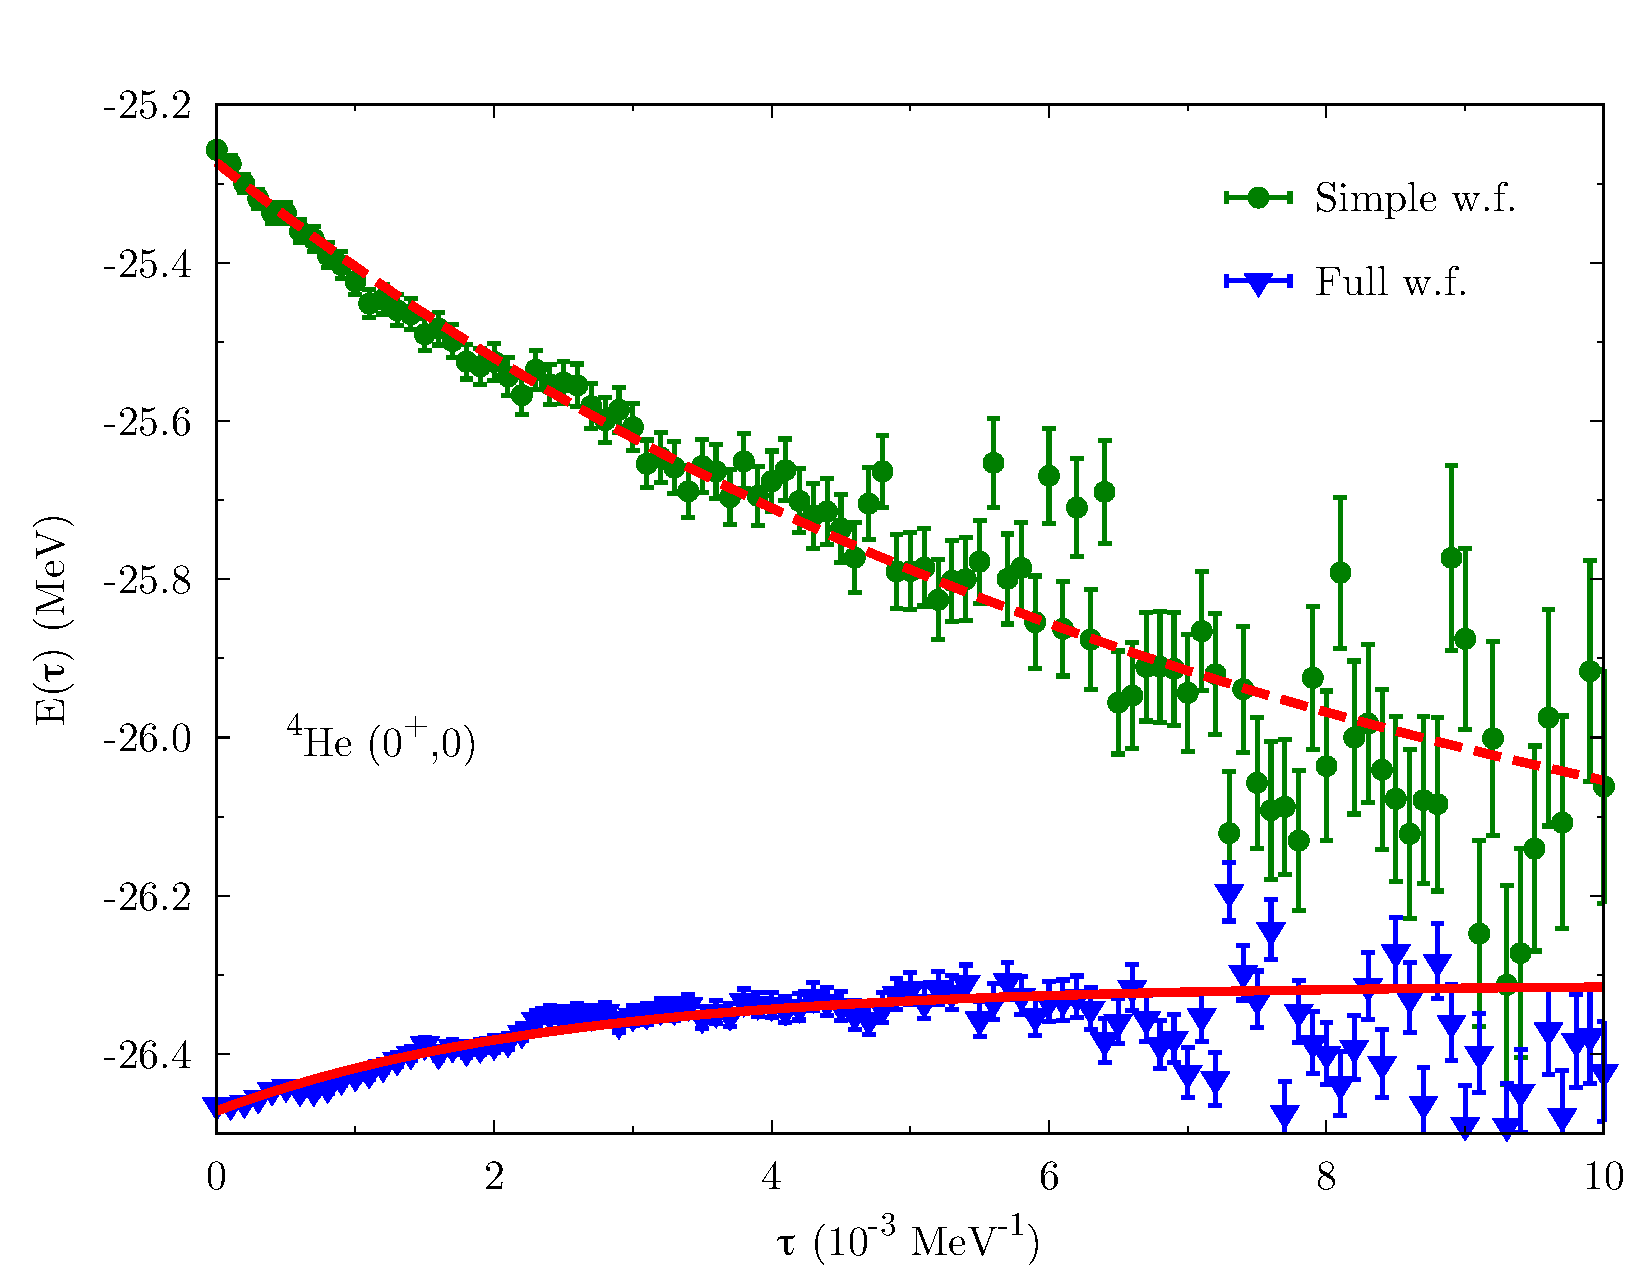
\includegraphics[width=\linewidth]{tr_he4.pdf}
\caption[]{Energy of \isotope[4]{He} as a function of the
imaginary time after releasing the constrain for the AV6$^\prime$ potential.}
\label{fig:tr_he4}
\end{figure}

We report in~\cref{tab:av6c} the constrained-path and unconstrained
energies for $A=3,4,6$ 
employing the AV6$^\prime$ potential, in comparison with the GFMC results for the same
interaction~\cite{Wiringa:2002}. It is interesting to note that constrained-path energies do not always satisfy 
the variational principle, as anticipated in~\cref{sec:cp}. This is seen, for example, in \isotope[3]{H}
and \isotope[4]{He}, for which the constrained-path energy is below the GFMC prediction, considered to be the 
exact solution for the given potential. However, once the unconstrained evolution is performed, 
AFDMC and GFMC results agree within 1\% or less.

\begin{table}[htb]
\centering
\caption[]{Ground state energies for $A=3,4,6$ employing the AV6$^\prime$ potential. Results are in MeV.}
\begin{tabular}{lccc}
\hline\hline
$\isotope[Z]{A}\,(J^\pi,T)$ & $E^{\rm CP}_{\rm AFDMC}$ & $E^{\rm U}_{\rm AFDMC}$ & $E_{\rm GFMC}$ \\
\hline
\isotope[3]{H}\,$(\frac{1}{2}^+,\frac{1}{2})$ & $-8.08(1)$  & $-7.95(2)$   & $-7.95(2)$  \\
\isotope[4]{He}\,$(0^+,0)$                    & $-26.45(1)$ & $-26.31(4)$  & $-26.15(2)$ \\
\isotope[6]{Li}\,$(1^+,0)$                    & $-28.09(4)$ & $-28.26(10)$ & $-28.37(4)$ \\
\hline\hline
\end{tabular}
\label{tab:av6c}
\end{table}

In~\cref{fig:tr_he6,fig:tr_o16} we show two examples of unconstrained calculation for larger systems,
\isotope[6]{He} and \isotope[16]{O} respectively, employing realistic two- plus three-body interactions. 
We use the local chiral potential at N$^2$LO with cutoff $R_0=1.2\,\rm fm$ for 
\isotope[6]{He} and $R_0=1.0\,\rm fm$ for \isotope[16]{O}. The employed wave functions include 
all two- and three-body correlations, and for \isotope[6]{He} we include single particle orbitals 
up to the $sd$ shell. In general, the larger the system, the shorter 
the imaginary time evolution that can be followed before the variance becomes 
too large. 
This is particularly evident in \isotope[16]{O} for which the unconstrained evolution 
can be satisfactorily performed up to $2.5\times10^{-4}\,\rm MeV^{-1}$, 
compared to the $4\times10^{-4}\,\rm MeV^{-1}$
for \isotope[6]{He} of~\cref{fig:tr_he6}, and to the $5\times10^{-3}\,\rm MeV^{-1}(10^{-2}\,\rm MeV^{-1})$ 
for \isotope[4]{He} with the same interaction (with AV6$^\prime$), \cref{fig:tr_he4}.
For example, at $\tau=2\times10^{-4}\,\rm MeV^{-1}$ the statistical error per nucleon is  
$0.01\,\rm MeV$ for \isotope[4]{He} and \isotope[6]{Li}, and $0.19\,\rm MeV$ for \isotope[16]{O}.
This is a direct consequence of the quality of the employed wave function. 
For small nuclei, the wave function of~\cref{eq:psi} provides a good description of the
system, and the constrained-path energy expectation value is already close to the expected result. 
In \isotope[6]{He} the difference between constrained and unconstrained energy is of 
the order of $1\,\rm MeV$, roughly $3\%$ of the final result. 
In \isotope[16]{O} instead, the constrained-path energy is higher, 
and the unconstrained evolution lowers 
its value of about $25\,\rm MeV$, $\approx22\%$ of the total energy.
This could be improved by employing more sophisticated wave functions including higher order
correlations, such as that of~\cref{eq:psi2}, 
and/or using more refined techniques to perform the unconstrained evolution. 
Studies along these directions are underway.

\begin{figure}[htb]
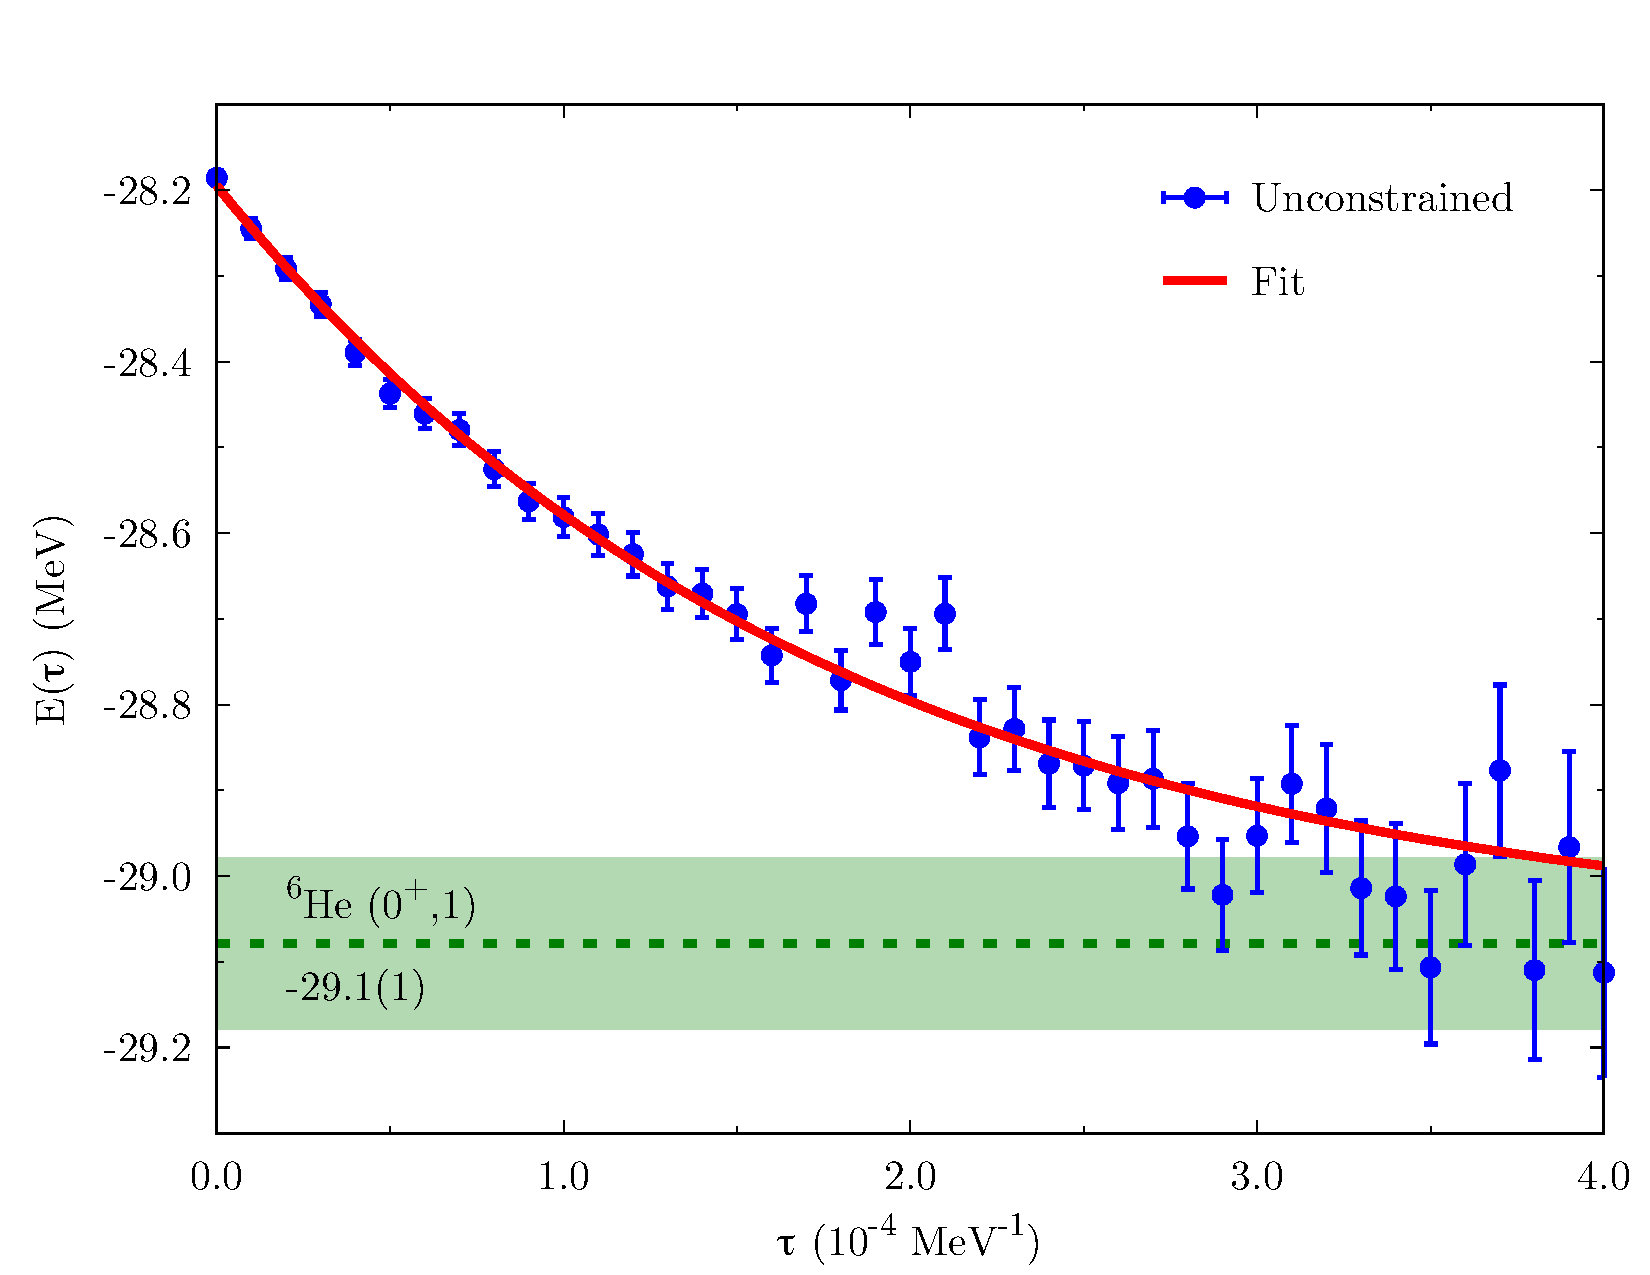
\includegraphics[width=\linewidth]{tr_he6.pdf}
\caption[]{\isotope[6]{He} unconstrained evolution for the local chiral potential at
N$^2$LO $(E\tau)$ with cutoff $R_0=1.2\,\rm fm$. Data points refer to the expectation 
value of $H'$, \cref{eq:h'}.}
\label{fig:tr_he6}
\end{figure}

\begin{figure}[htb]
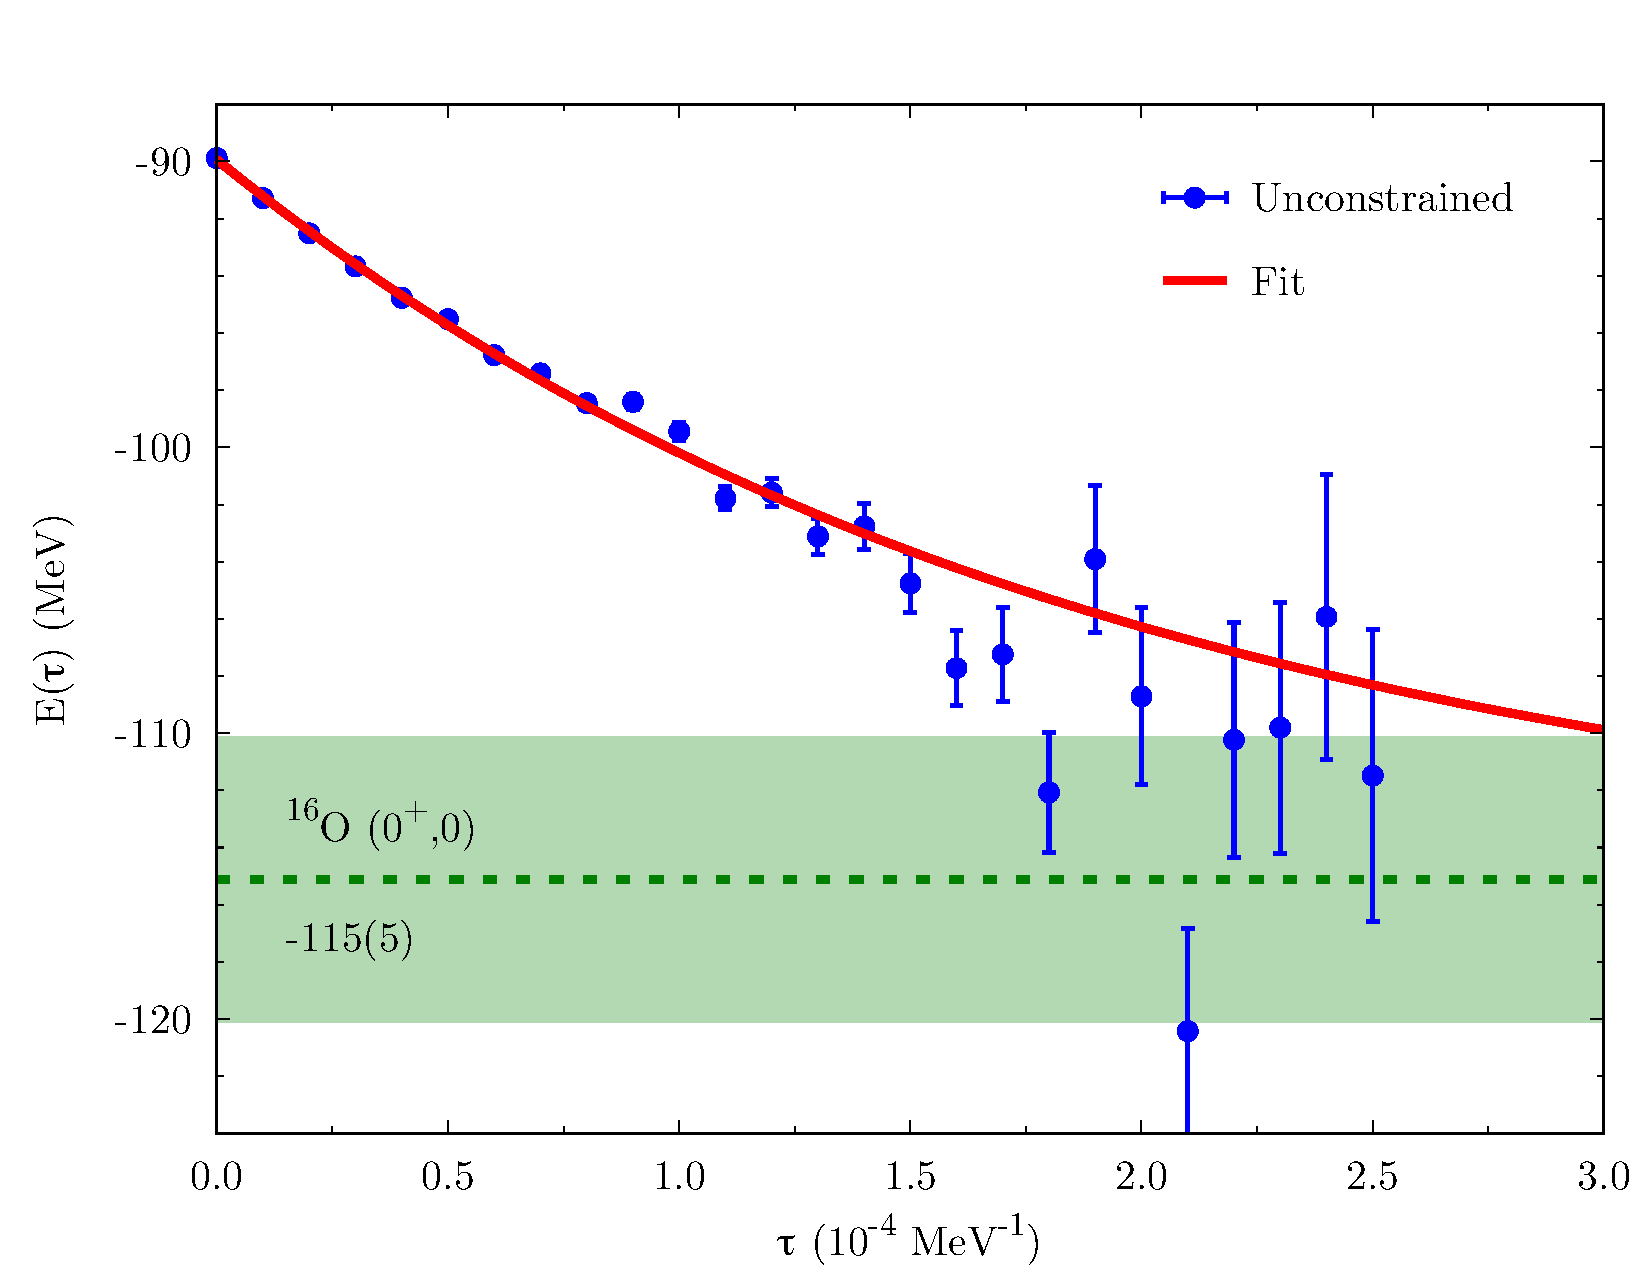
\includegraphics[width=\linewidth]{tr_o16.pdf}
\caption[]{\isotope[16]{O} unconstrained evolution for the local chiral potential at
N$^2$LO $(E\tau)$ with cutoff $R_0=1.0\,\rm fm$. Data points refer to the expectation 
value of $H'$, \cref{eq:h'}.}
\label{fig:tr_o16}
\end{figure}


\subsection{Test of quadratic two-body correlations}
\label{sec:psi2}
The results presented in the previous section are obtained using a trial wave function 
of the form~(\ref{eq:psi}), i.e. by retaining only two-body linear correlations in $\langle RS|\Psi\rangle$.
We present in~\cref{tab:psi2} a test study on the effect of including quadratic correlations
in the wave function to the energy expectation value. The constrained-path energies have been
calculated for \isotope[4]{He}, \isotope[16]{O}, and symmetric nuclear matter (SNM) with 28 particles 
in a box with periodic boundary conditions at saturation density $\rho_0=0.16$ fm$^{-3}$.
We use the AV6$^\prime$ potential with no Coulomb interaction for all the systems.
Results are shown for the linear, independent pair, and full quadratic two-body correlations.

\begin{table}[htb]
\centering
\caption[]{Energy per nucleon (in MeV) for \isotope[4]{He}, \isotope[16]{O}, and SNM at $\rho_0$.
The employed potential is AV6$^\prime$. No Coulomb interaction is considered here.
Results are shown for the linear, independent pair, and full quadratic two-body correlations.}
\begin{tabular}{ccccc}
\hline\hline
System & Linear & Ind-Pair & Quadratic \\
\hline
\isotope[4]{He} & -6.79(1)  & -6.81(1)  & -6.78(1)   \\
\isotope[16]{O} & -7.23(6)  & -7.59(9)  & -7.50(9)   \\
SNM             & -13.92(6) & -14.80(7) & -14.70(11) \\
\hline\hline
\end{tabular}
\label{tab:psi2}
\end{table}

Though there is little difference in \isotope[4]{He}, the constrained-path energies 
for both \isotope[16]{O} and SNM are lower when employing quadratic correlations, 
particularly for SNM. In \isotope[16]{O} the energy gain at the constrained-path
level is only $\approx0.3(1)\,\rm MeV/A$, while in SNM this value increases
up to $\approx0.8(1)\,\rm MeV/A$.
No difference is found, within statistical uncertainties, between independent pair
and full quadratic correlations results, except for the higher computational 
cost of the latter.
To be noted that the variational parameters in the trial wave function~(\ref{eq:psi2})
were re-optimized for \isotope[4]{He}. In the case of \isotope[16]{O} and SNM instead, 
due to the cost of optimizing such parameters using the full wave function of~\cref{eq:psi2},
we used the same parameters obtained for the linear wave function~(\ref{eq:psi}).


\subsection{\red{Fit of the three-body interaction}}
\red{Original reference}~\cite{Lynn:2016}

\begin{table}[htb]
\centering
\caption[]{C.}
\begin{tabular}{cccc}
\hline\hline
$V_{ijk}$    & $R_0\,(\rm fm)$ & $c_D$ & $c_E$ \\
\hline
$E\tau$      & $1.0$ & $0.0$   & $-0.63$ \\
             & $1.2$ & $3.5$   & $0.09$  \\
$E\mathbbm1$ & $1.0$ & $0.5$   & $0.62$  \\
             & $1.2$ & $-0.75$ & $0.025$ \\
\hline\hline
\end{tabular}
\label{tab:3bfit}
\end{table}

\begin{figure}[htb]
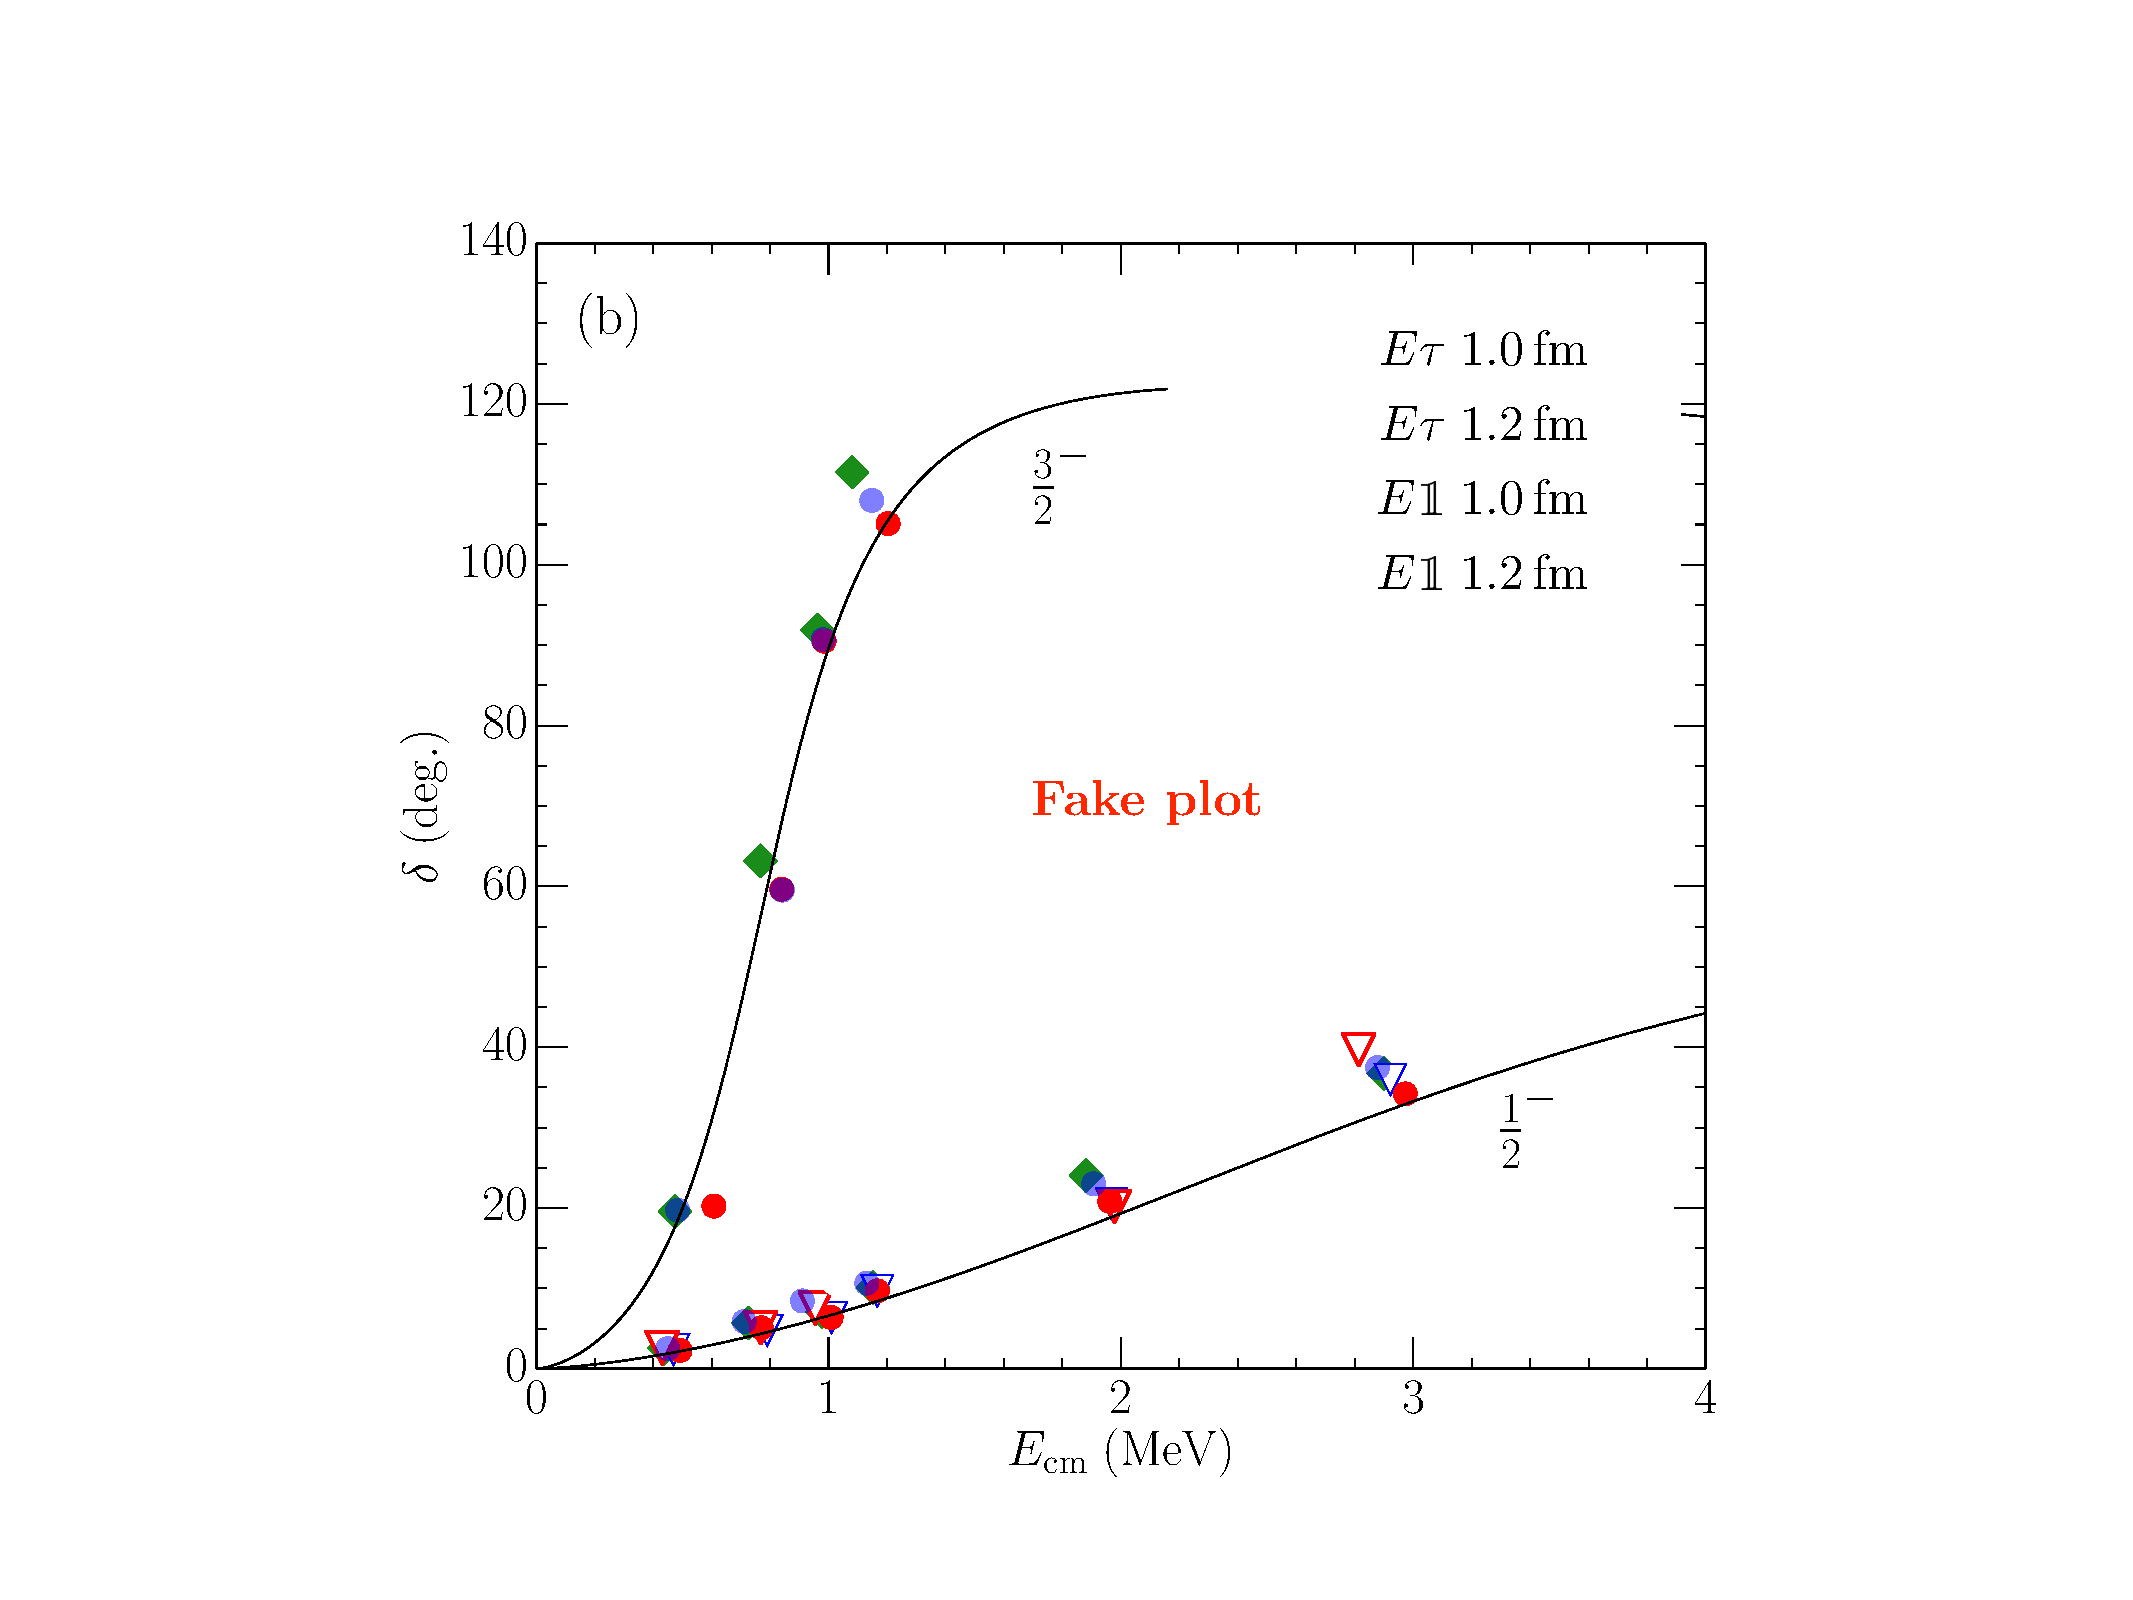
\includegraphics[width=\linewidth]{nalpha.pdf}
\caption[]{\red{Test image.}}
\label{fig:3bfit}
\end{figure}


\subsection{Test of the three-body calculation}
The energies reported in~\cref{fig:tr_he6,fig:tr_o16} correspond to the
expectation values of the effective Hamiltonian $H'$, \cref{eq:h'}. 
These need to be adjusted with the perturbative correction of~\cref{eq:<h3b>}---also extracted 
from the unconstrained evolution---in order to obtain the final results reported in~\cref{tab:10,tab:12}. 
Once the optimal set of parameters $\alpha_i$ is found, these corrections are small,
almost consistent with zero within Monte Carlo statistical uncertainties,
as shown in~\cref{tab:pert}.

\setlength{\tabcolsep}{4pt}
\begin{table}[htb]
\centering
\caption[]{Energy expectation values of~\cref{eq:<h3b>} for $A\ge6$. 
Results are in MeV.}
\begin{tabular}{lccccc}
\hline\hline
$\isotope[Z]{A}\,(J^\pi,T)$ & N$^2$LO & $R_0\,(\rm fm)$ & $\langle H'\rangle$ & $\langle V_{\rm pert}\rangle$ & $\langle H\rangle$ \\
\hline
\isotope[6]{He}\,$(0^+,1)$	& $E\tau$      & $1.0$ & $-28.3(4)$ & $0.1(2)$  & $-28.4(4)$ \\
							&              & $1.2$ & $-29.1(1)$ & $0.2(1)$  & $-29.3(1)$ \\
							& $E\mathbbm1$ & $1.0$ & $-28.5(5)$ & $-0.3(2)$ & $-28.2(5)$ \\
							&              & $1.2$ & $-$ & $$ & $-$ \\
\hline
\isotope[6]{Li}\,$(1^+,0)$	& $E\tau$      & $1.0$ & $-31.2(4)$ & $0.3(3)$  & $-31.5(5)$ \\
							&              & $1.2$ & $-31.9(3)$ & $0.4(1)$  & $-32.3(3)$ \\
							& $E\mathbbm1$ & $1.0$ & $-30.9(4)$ & $-0.2(2)$ & $-30.7(4)$ \\
							&              & $1.2$ & $-$ & $$ & $-$ \\
\hline
\isotope[12]{C}\,$(0^+,0)$	& $E\tau$      & $1.0$ & $-75(2)$ & $3(1)$ & $-78(3)$ \\
\hline                                     
\isotope[16]{O}\,$(0^+,0)$	& $E\tau$      & $1.0$ & $-115(5)$  & $2(1)$   & $-117(5)$  \\
							&              & $1.2$ & $-265(25)$ & $-2(6)$  & $-263(26)$ \\
							& $E\mathbbm1$ & $1.0$ & $-$ & $$ & $-$ \\
							&              & $1.2$ & $-$ & $$ & $-$ \\
\hline\hline
\end{tabular}
\label{tab:pert}
\end{table}
\setlength{\tabcolsep}{10pt}

The final result $\langle H\rangle$ is, however, nearly independent to variations
of the $\alpha_i$ parameters, even for larger systems. This is shown in~\cref{tab:alpha} 
where the $\alpha_i$ are arbitrarily changed in \isotope[16]{O} within $5-10$\% with respect 
to the optimal values, given in the first row for each cutoff. 
This results in $\lesssim4$\% variations of the total energy, 
compatible with the overall Monte Carlo statistical uncertainties. 
To be noted that, in order to save computing time, this test has been done using the 
constrained-path evolution. However, the optimal constrained-path expectation values 
$\langle V_{\rm pert}\rangle$ are consistent with the unconstrained ones of~\cref{tab:pert}.

\setlength{\tabcolsep}{1.5pt}
\begin{table}[htb]
\centering
\caption[]{Contributions to the energy expectation value of~\cref{eq:<h3b>} in \isotope[16]{O}.
The parametrization $E\tau$ of the three-body force is used for different cutoffs.
$\langle V_{\rm pert}\rangle$ is the proper mixed estimator. 
For each cutoff, the first line represents the optimal choice for $\alpha_i$.
Energies (in MeV) are the result of the constrained-path evolution.}
\begin{tabular}{ccccc}
\hline\hline
$R_0\,(\rm fm)$ & $(\alpha_1,\alpha_2,\alpha_3)$ & $\langle H'\rangle$ & $\langle V_{\rm pert}\rangle$ & $\langle H\rangle$ \\
\hline
$1.0$ & $(2.05,-3.80,-0.95)$ & $-90.0(3)$  & $1.8(5)$    & $-91.8(6)$   \\
      & $(2.50,-3.30,-1.20)$ & $-125.1(6)$ & $-33.9(8)$  & $-92.2(1.0)$ \\
      & $(1.95,-4.00,-0.90)$ & $-83.3(2)$  & $5.9(9)$    & $-89.2(1.0)$ \\
%     & $(2.15,-4.00,-1.00)$ & $-91.4(4)$  & $0.5(1.2)$  & $-92.0(1.2)$ \\
%     & $(1.95,-3.60,-0.90)$ & $-87.4(6)$  & $5.2(1.1)$  & $-92.6(1.3)$ \\
      & $(1.80,-4.20,-0.85)$ & $-75.6(3)$  & $13.9(1.4)$ & $-89.4(1.5)$ \\
\hline                        
$1.2$ & $(1.80,0.45,8.00)$   & $-171(2)$   & $-2(1)$     & $-169(2)$    \\
      & $(1.90,0.50,8.50)$   & $-197(3)$   & $-25(2)$    & $-172(3)$    \\
      & $(1.70,0.40,7.50)$   & $-147(1)$   & $15(1)$     & $-162(1)$    \\
%     & $(2.00,0.35,9.00)$   & $-177(2)$   & $7(1)$      & $-184(2)$    \\
\hline\hline
\end{tabular}
\label{tab:alpha}
\end{table}
\setlength{\tabcolsep}{10pt}

Unless differently specified, in the following all ground state energies will 
correspond to the final expectation value $\langle H\rangle$, extracted from 
the unconstrained Monte Carlo results for $\langle H'\rangle$ with an exponential fit, 
and adjusted with the perturbative correction of~\cref{eq:<h3b>} when three-body forces are employed.


\subsection{Ground state energies and charge radii}
We consider local chiral Hamiltonians at leading-order (LO), 
next-to-leading-order (NLO), and N$^2$LO, the latter including both two- and three-body forces.
At each order we can assign theoretical uncertainties to observables coming from the 
truncation of the chiral expansion~\cite{Epelbaum:2015epja}. For an observable $X$ at N$^2$LO, 
the theoretical uncertainty is obtained as
\begin{align}
\Delta X^{\text{N}^2\text{LO}}=&\max(Q^4\times|X^{\text{LO}}|,\nonumber \\ 
&\phantom{\max(\,}Q^2\times|X^{\text{NLO}}-X^{\text{LO}}|, \nonumber \\
&\phantom{\max(\,}Q^{\phantom{2}}\times|X^{\text{N}^2\text{LO}}-X^{\text{NLO}}|),
\label{eq:err}
\end{align}
where we take $Q=m_\pi/\Lambda_b$ with $m_\pi\approx140\,\rm MeV$ and $\Lambda_b=600$~MeV, 
as done in~\cite{Lynn:2016,Lonardoni:2017afdmc}.

The expectation value of the charge radius is derived from the point-proton radius using the relation:
\begin{align}
	\left\langle r_{\rm ch}^2\right\rangle=
	\left\langle r_{\rm pt}^2\right\rangle+
	\left\langle R_p^2\right\rangle+
	\frac{A-Z}{Z}\left\langle R_n^2\right\rangle+
	\frac{3\hbar^2}{4M_p^2c^2},
	\label{eq:rch}
\end{align}
where $r_{\rm pt}$ is the calculated point-proton radius,
$\left\langle R_p^2\right\rangle=0.770(9)\,\rm{fm}^2$~\cite{Beringer:2012} the proton radius, 
$\left\langle R_n^2\right\rangle=-0.116(2)\,\rm{fm}^2$~\cite{Beringer:2012} the neutron radius,
and $(3\hbar^2)/(4M_p^2c^2)\approx0.033\,\rm{fm}^2$ the Darwin-Foldy correction~\cite{Friar:1997}.
For \isotope[6]{He} a spin-orbit correction 
$\left\langle r_{\rm so}^2\right\rangle=-0.08\,\rm{fm}^2$~\cite{Ong:2010} is also included.
The point-nucleon radius $r_{\rm pt}$ is calculated as
\begin{align}
	\left\langle r_N^2\right\rangle=\frac{1}{{\cal N}}\big\langle\Psi\big|\sum_i\mathcal P_{N_i} |\vb{r}_i-\vb{R}_{\rm cm}|^2\big|\Psi\big\rangle,
\end{align}
where $\vb{R}_{\rm cm}$ is the coordinate of the center of mass of the system,
${\cal N}$ is the number of protons or neutron, and 
\begin{align}
	\mathcal P_{N_i}=\frac{1\pm\tau_{z_i}}{2},
	\label{eq:proj}
\end{align}
is the projector operator onto protons or neutrons. 
The charge radius is a mixed expectation value, and it requires the calculation of both
VMC and DMC point-proton radii, accordingly to~\cref{eq:mix}. 
Regardless the employed optimization of the variational wave function (free or constrained), 
the extrapolation of the mixed estimate $\left\langle r_{\rm ch}^2\right\rangle$ is small, 
and the final results are typically within statistical uncertainties.

The ground state energies and charge radii for light systems $(A=3,4)$ employing 
the local chiral potential at N$^2$LO are shown in~\cref{tab:afdmc-gfmc}. 
Results with ($E\tau$ parametrization) and without the three-body force are shown 
for different choices of the cutoff $R_0$. For all the $s_{1/2}$ systems we used the same 
parameters $\alpha_i$ for the propagation of the three-body force, 
determined in order to minimize the perturbative correction of~\cref{eq:<h3b>}.
The agreement with the GFMC results of Ref.~\cite{Lynn:2016,Lynn:2017},
where the three-body interactions are fully included in the propagation, 
is within few percent both at the two- and three-body level, providing a good
benchmark for the AFDMC propagation technique described in~\cref{sec:p3}.

\begin{table*}[htb]
\centering
\caption[]{Ground state energies and charge radii for $A=3,4$ employing the local chiral potential at N$^2$LO. 
The $E\tau$ parametrization is used for the three-body force.
GFMC results are from Refs.~\cite{Lynn:2014,Lynn:2016}.}
\begin{tabular}{cclcccc}
\hline\hline
Nucleus                     & Cutoff     & Potential & \multicolumn{2}{c}{AFDMC}      & \multicolumn{2}{c}{GFMC} \\
$\isotope[Z]{A}\,(J^\pi,T)$ & $R_0$ (fm) &           &  $E$ (MeV) & $r_{\rm ch}$ (fm) & $E$ (MeV) & $r_{\rm ch}$ (fm) \\     
\hline
\isotope[3]{H}\,$(\frac{1}{2}^+,\frac{1}{2})$  & $1.0$ & 2b    & $-7.54(4)$   & $1.75(2)$ & $-7.55(1)$  & $1.78(2)$ \\
   	  	                                       &       & 2b+3b & $-8.33(7)$   & $1.72(2)$ & $-8.34(1)$  & $1.72(3)$ \\
                                               & $1.2$ & 2b    & $-7.76(3)$   & $1.74(2)$ & $-7.74(1)$  & $1.75(2)$ \\
   	  	                                       &       & 2b+3b & $-8.27(5)$   & $1.73(2)$ & $-8.35(4)$  & $1.72(4)$ \\
\hline                                                                    
\isotope[3]{He}\,$(\frac{1}{2}^+,\frac{1}{2})$ & $1.0$ & 2b    & $-6.89(5)$   & $2.02(2)$ & $-6.78(1)$  & $2.06(2)$ \\
                                               &       & 2b+3b & $-7.55(8)$   & $1.96(2)$ & $-7.65(2)$  & $1.97(2)$ \\
                                               & $1.2$ & 2b    & $-7.12(3)$   & $1.98(2)$ & $-7.01(1)$  & $2.01(1)$ \\
                                               &       & 2b+3b & $-7.64(4)$   & $1.95(5)$ & $-7.63(4)$  & $1.97(1)$ \\
\hline                                               
\isotope[4]{He}\,$(0^+,0)$                     & $1.0$ & 2b    & $-23.96(8)$  & $1.72(2)$ & $-23.72(1)$ & $1.73(1)$ \\
                                               &       & 2b+3b & $-27.64(13)$ & $1.68(2)$ & $-28.30(1)$ & $1.65(2)$ \\
                                               & $1.2$ & 2b    & $-25.17(5)$  & $1.69(1)$ & $-24.86(1)$ & $1.69(1)$ \\
                                               &       & 2b+3b & $-28.37(8)$  & $1.65(1)$ & $-28.30(1)$ & $1.64(1)$ \\
\hline\hline
\end{tabular}
\label{tab:afdmc-gfmc}
\end{table*}

In~\cref{fig:ene_10,fig:ene_12} we present the ground state energies per nucleon
of nuclei with $3\le A\le16$ for cutoffs $R_0=1.0\,\rm fm$ and $R_0=1.2\,\rm fm$, 
respectively. Results at LO, NLO, and N$^2$LO for both $E\tau$ and $E\mathbbm1$
parametrizations of the three-body force are shown. Error bars are estimated by 
including both the Monte Carlo uncertainties and the errors given by 
the truncation of the chiral expansion, the latter being the dominant ones.
For the hard interaction $(R_0=1.0\,\rm fm)$, the predicted binding energies at N$^2$LO 
are in good agreement with experimental data all the way up to $A=16$.
No differences, within error bars, are found for the two different
parametrizations of the three-body force.

\isotope[12]{C} in the $E\tau$ parametrization is slightly underbound.
This is most likely a consequence of the employed wave function that results 
in a too high constrained-path energy. 
This could be due to the complicated clustering structure of $^{12}$C not included
in $\Psi_T$, that would require a much longer unconstrained propagation
to filter out the corresponding low excitations from $\Psi_T$.
For $A=6$ the wave
function is constructed using up to $sd$ shell single-particle orbitals. For \isotope[12]{C} 
instead, coupling $p$ shell orbitals only
already results in a sum of 119 Slater determinants. Including orbitals in the $sd$ shell could 
in principle result in a better wave function for this open-shell system, but it will 
sizably increase the number of determinants to consider, making the calculation prohibitively 
time consuming. Another possible improvement would be to include quadratic terms in
the pair correlations, as shown in~\cref{eq:psi2}. However, first attempts in
\isotope[16]{O} lead to just a $\approx6(2)\,\rm MeV$ reduction of the total 
energy in a simplified scenario (see~\cref{tab:psi2}), with a noticeably increase of 
computational cost.

\begin{figure}[t]
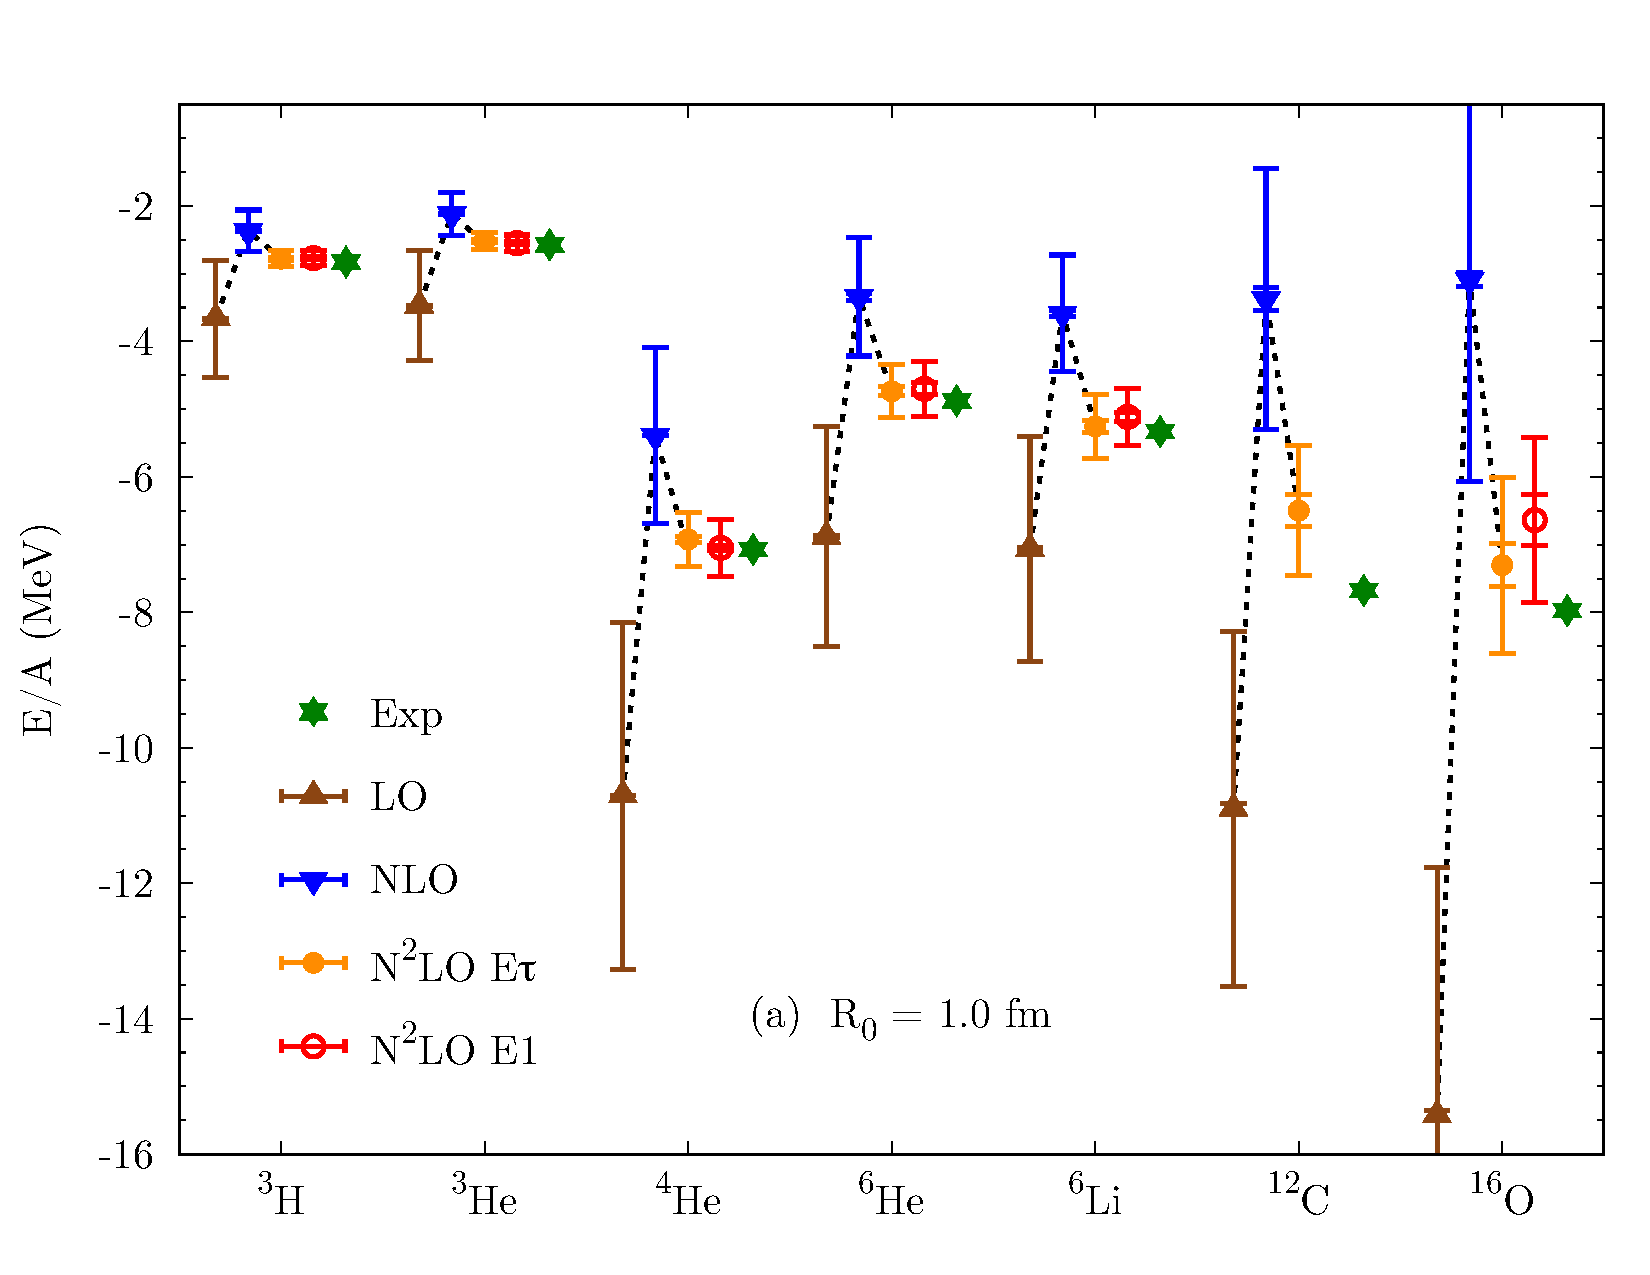
\includegraphics[width=\linewidth]{ene_10.pdf}
\caption[]{Ground state energies per nucleon for $3\le A\le16$ with the local chiral potential 
for the $R_0=1.0\,\rm fm$ cutoff. Results at different order of the chiral expansion and for 
different three-body parametrizations are shown.
Smaller error bars (indistinguishable from the symbols up to $A=6$) 
indicate the statistical Monte Carlo uncertainty,
while larger error bars are the uncertainties from the truncation of
the chiral expansion. Updated from Ref.~\cite{Lonardoni:2017afdmc}.}
\label{fig:ene_10}
\end{figure}

\begin{figure}[t]
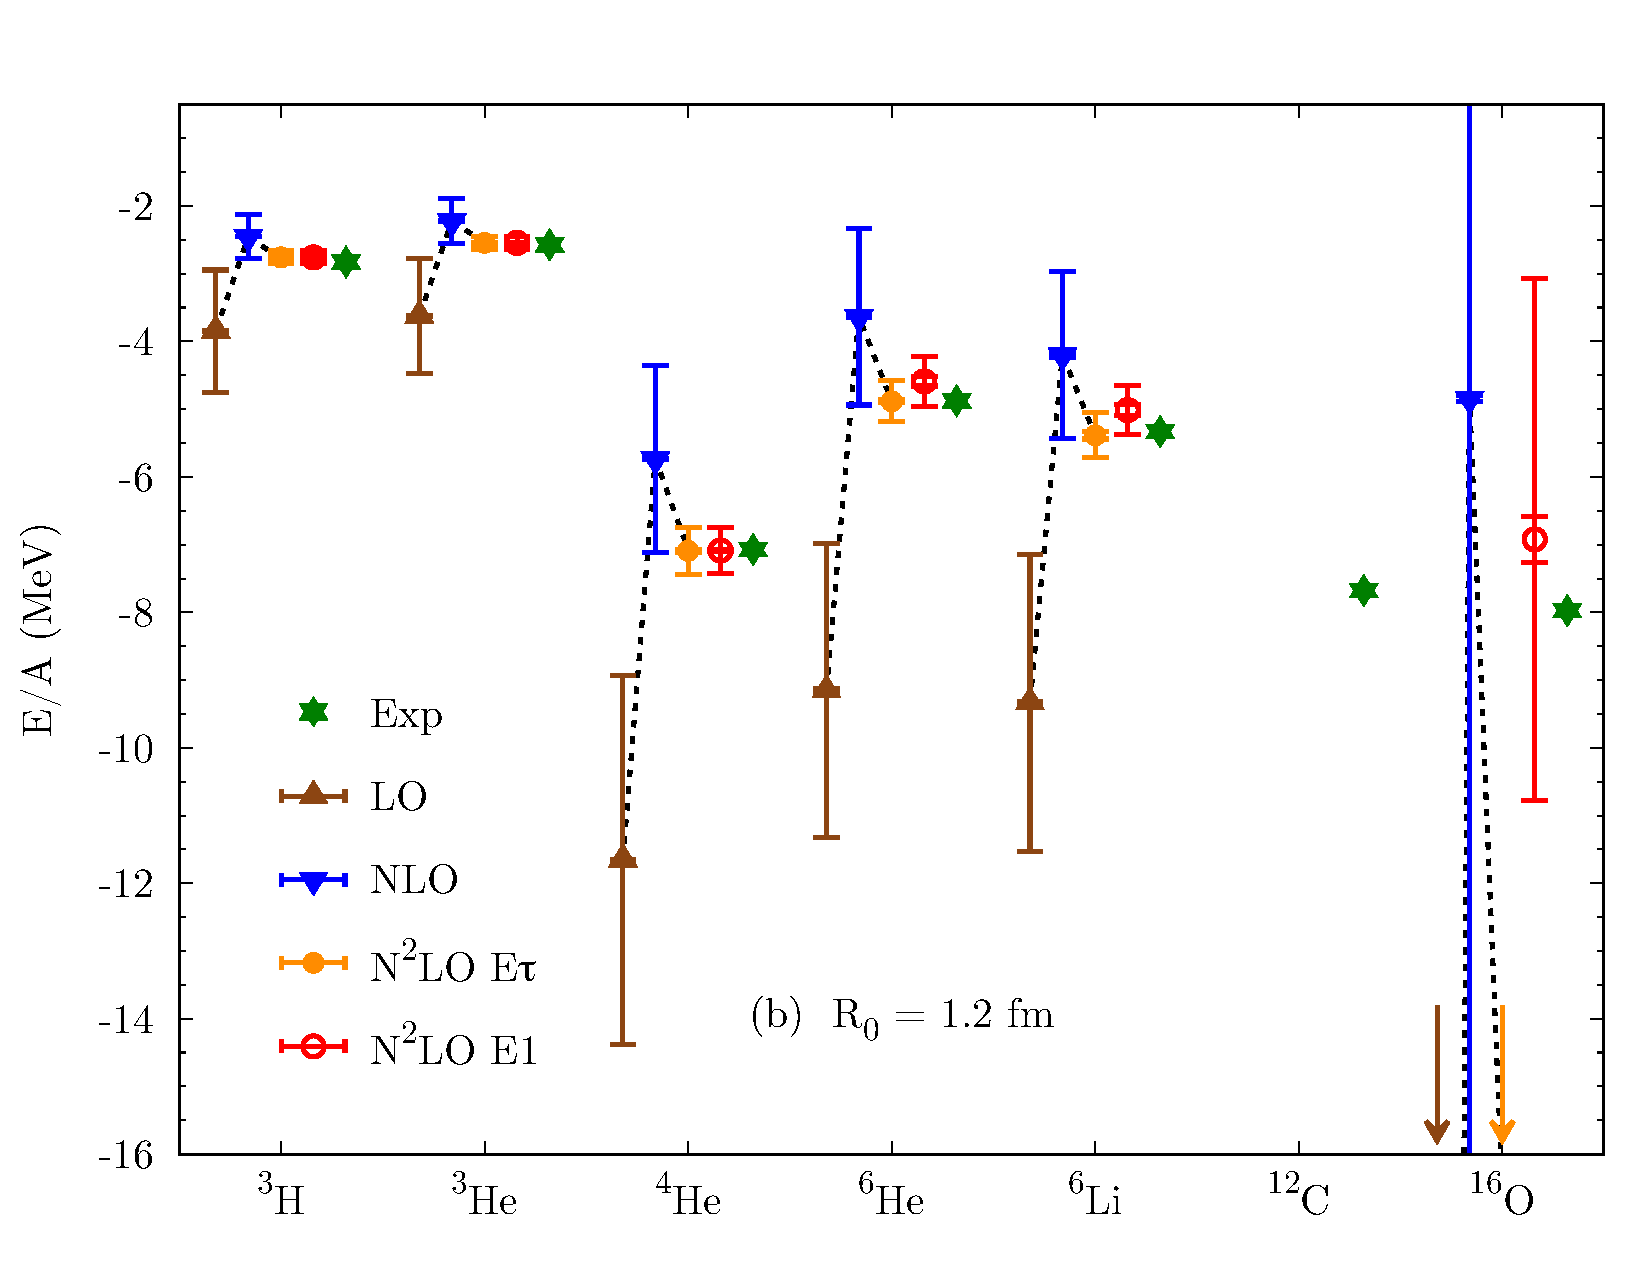
\includegraphics[width=\linewidth]{ene_12.pdf}
\caption[]{Same of~\cref{fig:ene_10} but for the $R_0=1.2\,\rm fm$ cutoff.
LO and N$^2$LO $E\tau$ results for \isotope[16]{O} are outside the displayed energy region.}
\label{fig:ene_12}
\end{figure}

For the soft interaction $(R_0=1.2\,\rm fm)$, NLO and in particular LO results are 
typically more bound compared to the $R_0=1.0\,\rm fm$ case. Both parametrizations
of the three-body force bring the N$^2$LO energies compatible with the experimental 
values up to $A=6$, and consistent with those obtained with the hard potential. 
\red{(to be verified in \isotope[6]{He} and \isotope[6]{Li}).}

Different is the case of \isotope[16]{O} that at LO is dramatically overbound
$(\approx -1\,\rm GeV)$, implying huge theoretical errors at NLO and N$^2$LO coming from 
the prescription of~\cref{eq:err}. Within these uncertainties, NLO and N$^2$LO two-body energies 
are compatible with the corresponding results for the hard interaction (see~\cref{tab:10,tab:12}).
However, the contribution of the three-body force at N$^2$LO largely depends upon
the employed operator structure. The $E\tau$ parametrization for the soft potential is very attractive,
adding almost $10\,\rm MeV$ per nucleon to the total energy, and thus
predicting a severe overbinding with a ground state energy of $\approx -260\,\rm MeV$.
The $E\mathbbm1$ parametrization is instead less attractive, resulting in a $0.3\,\rm MeV$ per 
nucleon more binding with respect to the two-body case \red{(to be verified)}, result compatible
with the energy expectation values for the hard interaction.
It follows that softer local Hamiltonians manifest issues in the description of medium-mass nuclei, 
calling for a significant dependence on the employed operator structure 
and, possibly, for the necessity of inputs other than few-body observables, as already pointed out 
for example in Ref.~\cite{Ekstrom:2015}.

\Cref{fig:rch_10,fig:rch_12} show the charge radii at different orders of the chiral 
expansion and for different cutoffs and parametrizations of the three-body force. 
The agreement with experimental data for the hard interaction at N$^2$LO is remarkably
good all the way up to oxygen. Exception is \isotope[6]{Li}, for which the charge radius
is somewhat underpredicted. However, a similar conclusion is found in GFMC calculations
employing the AV18+IL7 potential, where charge radii of lithium isotopes are underestimated. 

For the soft interaction, the description of charge radii resembles order by order 
that for the hard potential up to \isotope[4]{He}, with the N$^2$LO results in agreement 
with experimental data (also shown in~\cref{tab:afdmc-gfmc}). 
The picture changes instead for $A\ge6$, with radii progressively smaller at each order
compared to the $R_0=1.0\,\rm fm$ case, and no longer compatible at N$^2$LO with experimental 
values. The charge radius of \isotope[16]{O} turns out to be close to $2.2\,\rm fm$ with the 
soft interaction, smaller than that of \isotope[6]{Li} for the same potential, 
but consistent with the severe overbinding predicted for $A=16$.
\red{(need the new results for $E\mathbbm1$ to complete this paragraph).}

\begin{figure}[htb]
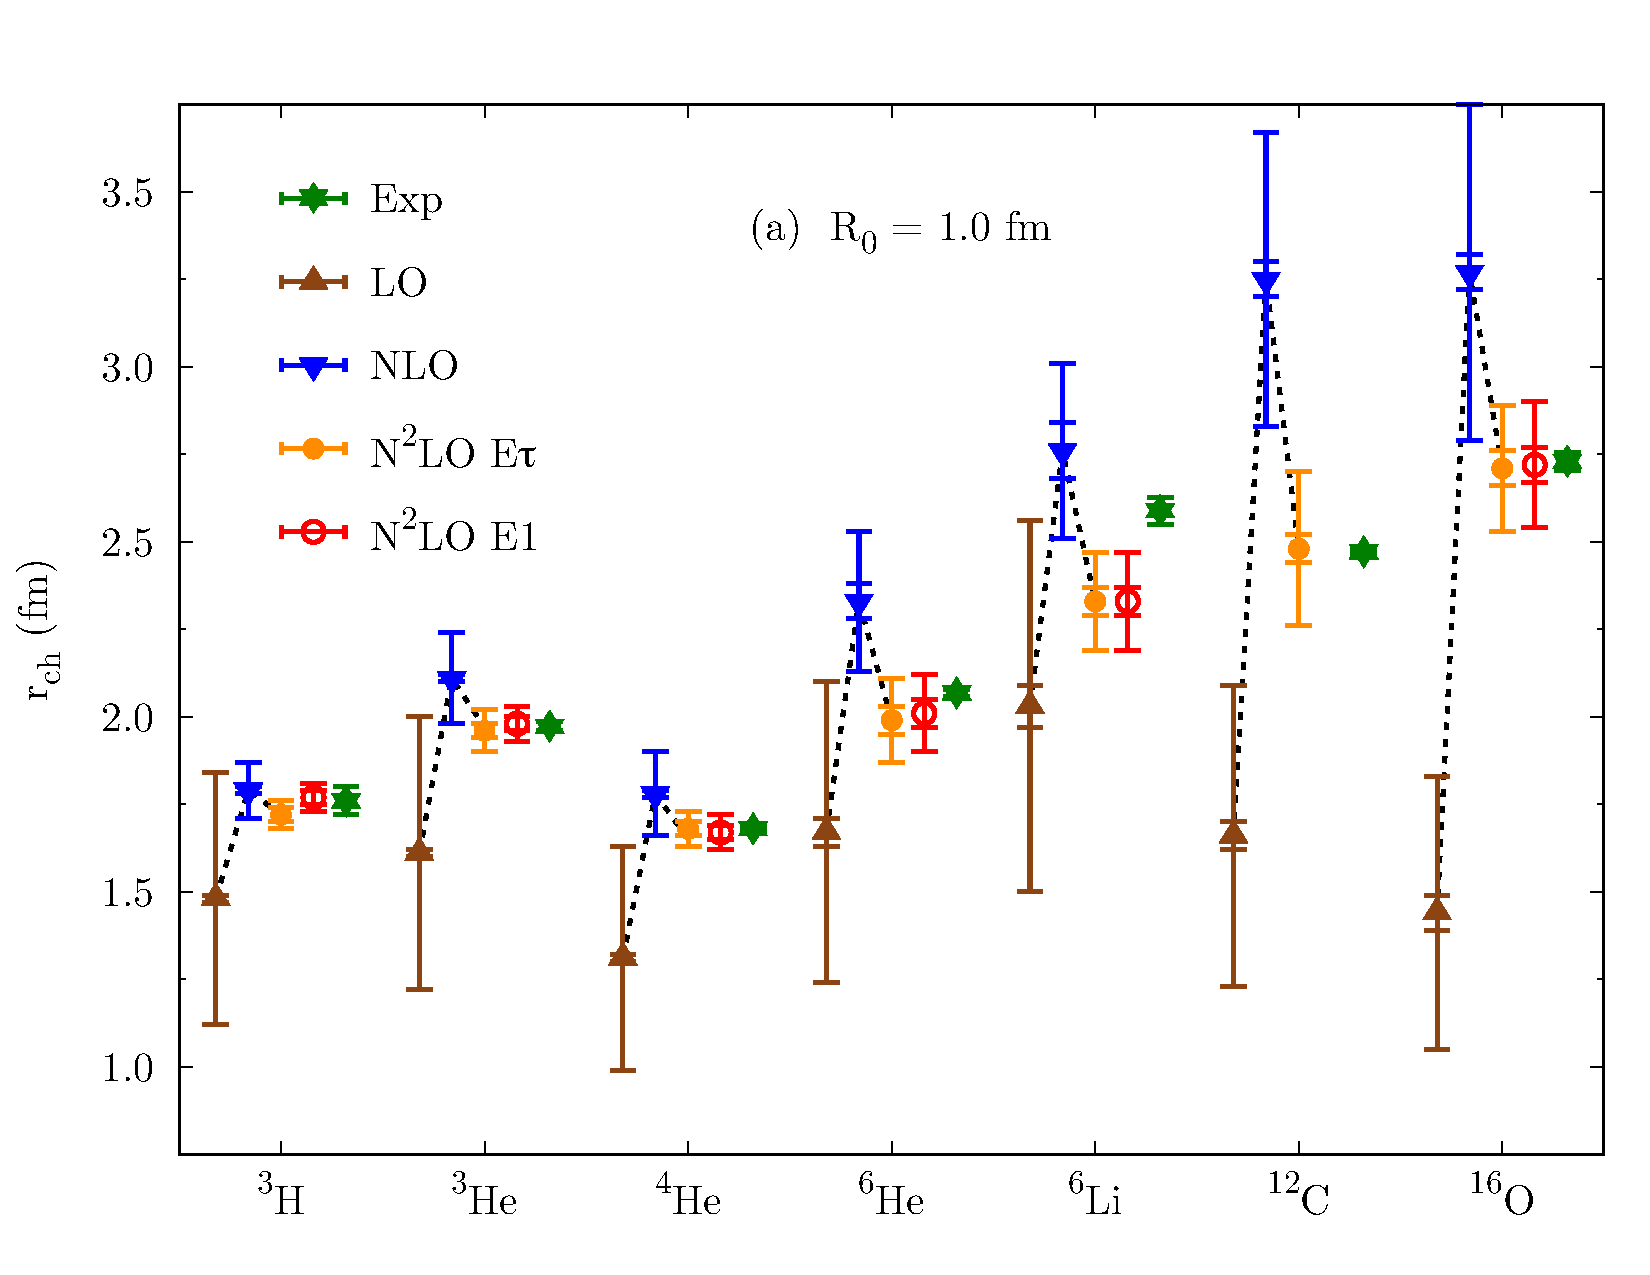
\includegraphics[width=\linewidth]{rch_10.pdf}
\caption[]{Charge radii for $3\le A\le16$ with the local chiral potential 
for the $R_0=1.0\,\rm fm$ cutoff. Results at different order of the chiral expansion 
and for different three-body parametrizations are shown.
Error bars are as in~\cref{fig:ene_10}. Updated from Ref.~\cite{Lonardoni:2017afdmc}.}
\label{fig:rch_10}
\end{figure}

\begin{figure}[htb]
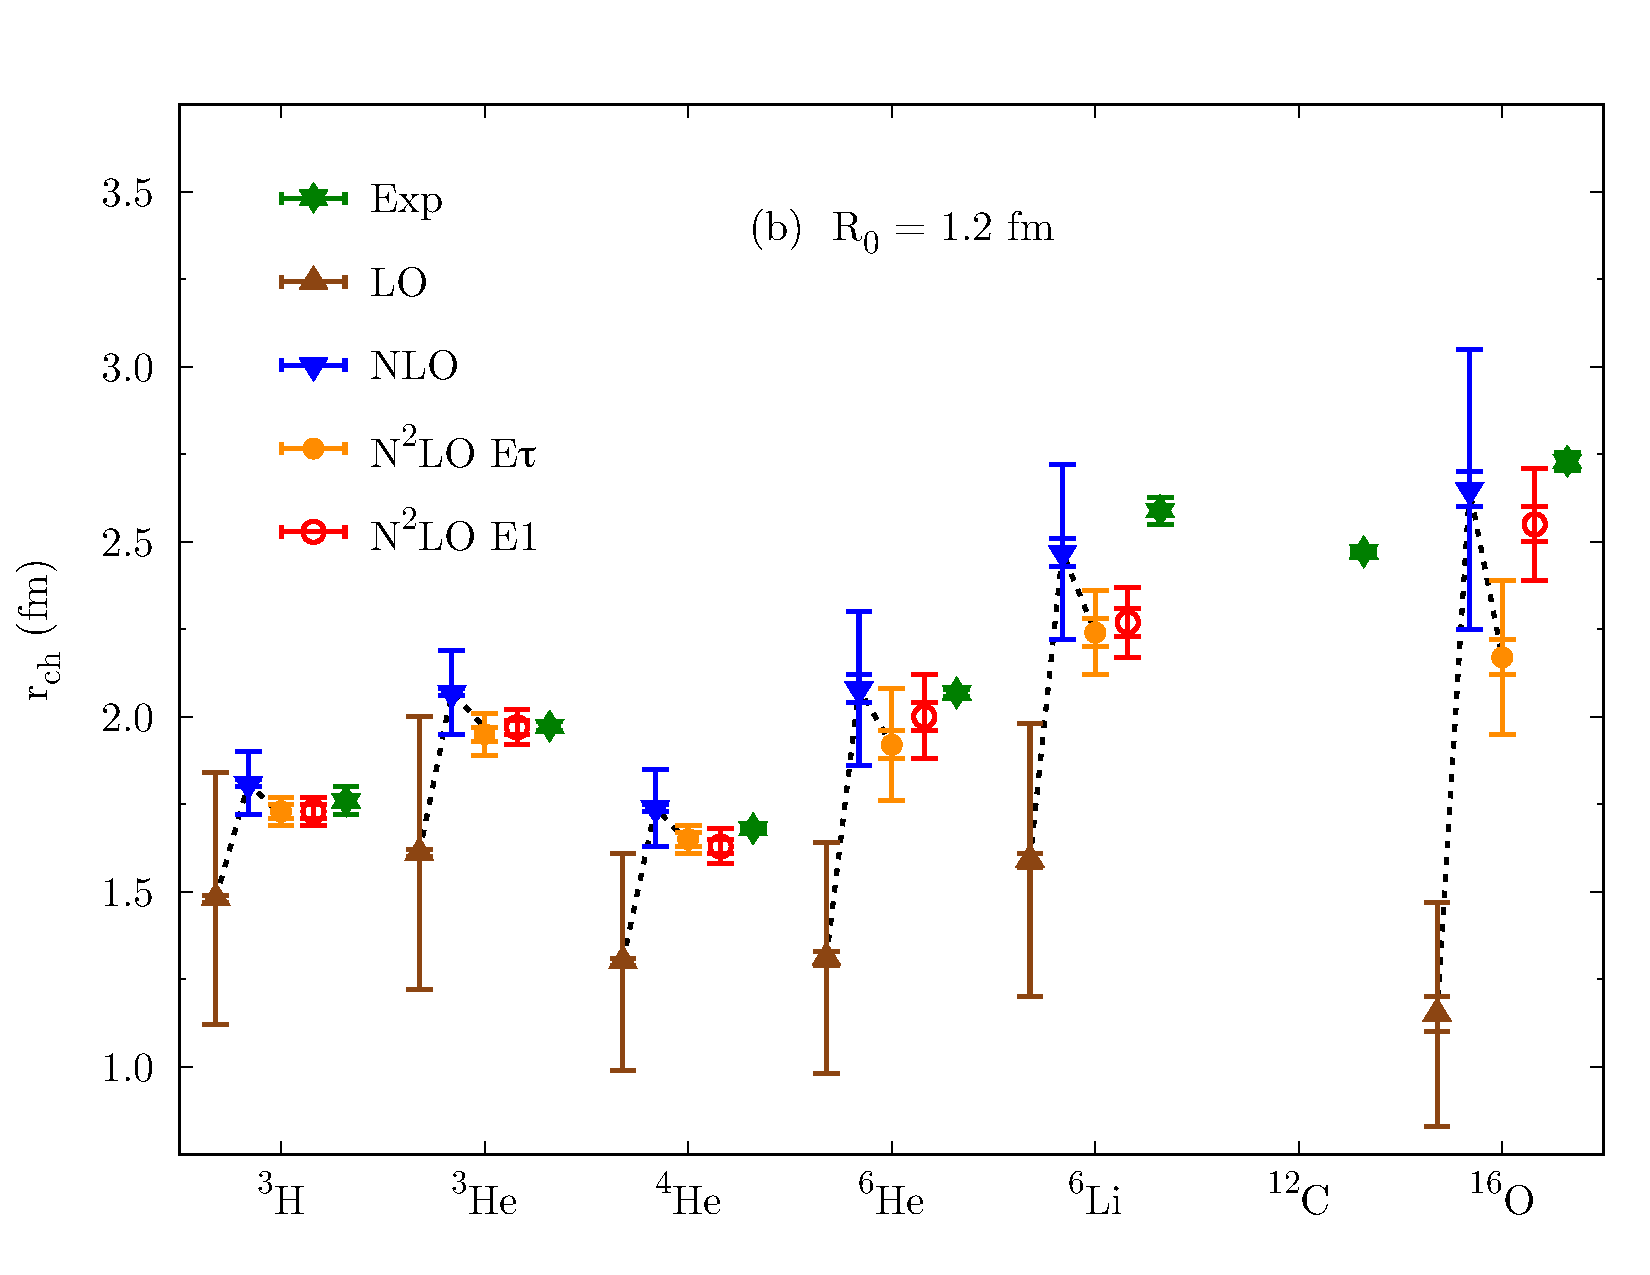
\includegraphics[width=\linewidth]{rch_12.pdf}
\caption[]{Same as~\cref{fig:rch_10} but for the $R_0=1.2\,\rm fm$ cutoff.}
\label{fig:rch_12}
\end{figure}

The details of LO, NLO, and N$^2$LO calculations for $A\ge6$ are reported in~\cref{tab:10,tab:12}
for $R_0=1.0\,\rm fm$ and $R_0=1.2\,\rm fm$, respectively. Results for the constrained-path and 
unconstrained evolution energies are both shown, together with the charge radius.
Both Monte Carlo uncertainties and theoretical errors coming from the truncation of the chiral 
expansion are reported (where available). At N$^2$LO the two-body energy is shown together with
that of two different parametrizations of the three-body force ($E\tau$ and $E\mathbbm{1}$).

The full calculation of \isotope[12]{C} at N$^2$LO required 
order of $10^6$ CPU hours (on Intel Broadwell cores @ 2.1GHz) for a single cutoff $(1.0\,\rm fm)$ 
and three-body parametrization $(E\tau)$. Due to the high computational cost, no attempts were
made for the $E\mathbbm{1}$ parametrization of the three-body force or for the $1.2\,\rm fm$ cutoff.

\begin{table*}[htb]
\centering
\caption[]{Ground state energies and charge radii for $A\ge6$ with the local chiral potential. 
Results at different order of the chiral expansion and for different three-body parametrizations are shown. 
$E_{\rm CP}$ is the constrained-path energy, while $E$ refers to the unconstrained evolution.
The first error is statistical, the second systematic.
The employed cutoff is $R_0=1.0\,\rm fm$.}
\begin{tabular}{llccc}
\hline\hline
$\isotope[Z]{A}\,(J^\pi,T)$ & Potential & $E_{\rm CP}$ (MeV) & $E$ (MeV) & $r_{\rm ch}$ (fm) \\
\hline                                         
\isotope[6]{He}\,$(0^+,1)$                     & LO                     & $-42.1(1)$  & $-41.3(1)(9.6)$ & $1.67(4)(39)$ \\
                                               & NLO                    & $-18.19(7)$ & $-20.0(3)(5.0)$ & $2.33(5)(15)$ \\
                                               & N$^2$LO 2b             & $-22.24(4)$ & $-23.1(2)(1.2)$ & $2.11(4)(5)$ \\
   	  	                                       & N$^2$LO $E\tau$        & $-26.58(6)$ & $-28.4(4)(2.0)$ & $1.99(4)(8)$ \\
   	  	                                       & N$^2$LO $E\mathbbm{1}$ & $-26.33(8)$ & $-28.2(5)(1.9)$ & $2.01(4)(7)$ \\
                                               & exp                    &             & $-29.3$         & $2.07$        \\
\hline                                                                  
\isotope[6]{Li}\,$(1^+,0)$                     & LO                     & $-42.8(1)$  & $-42.4(1)(9.9)$ & $2.03(6)(47)$ \\
                                               & NLO                    & $-19.2(2)$  & $-21.5(3)(4.9)$ & $2.76(8)(17)$ \\
                                               & N$^2$LO 2b             & $-24.3(1)$  & $-25.5(4)(1.1)$ & $2.46(4)(7)$  \\
   	  	                                       & N$^2$LO $E\tau$        & $-28.9(1)$  & $-31.5(5)(2.3)$ & $2.33(4)(10)$ \\
   	  	                                       & N$^2$LO $E\mathbbm{1}$ & $-28.9(1)$  & $-30.7(4)(2.1)$ & $2.33(4)(10)$ \\
                                               & exp                    &             & $-32.0$         & $2.59(4)$     \\
\hline                                                                  
\isotope[12]{C}\,$(0^+,0)$                     & LO                     & $-131.5(2)$ & $-131(1)(31)$   & $1.66(4)(39)$ \\
                                               & NLO                    & $-31.1(2)$  & $-41(2)(21)$    & $3.25(5)(37)$ \\
                                               & N$^2$LO 2b             & $-63.5(2.4)$& $-66(3)(6)$     & $2.66(4)(14)$ \\
   	  	                                       & N$^2$LO $E\tau$        & $-70.2(5)$  & $-78(3)(9)$     & $2.48(4)(18)$ \\
   	  	                                       & N$^2$LO $E\mathbbm{1}$ & $-$         & $-$             & $-$           \\
                                               & exp                    &             & $-92.2$         & $2.47$        \\
\hline                                                                  
\isotope[16]{O}\,$(0^+,0)$                     & LO                     & $-251.7(2)$ & $-247(1)(58)$   & $1.44(3)(34)$ \\
                                               & NLO                    & $-37.3(2)$  & $-49(2)(46)$    & $3.27(5)(43)$ \\
                                               & N$^2$LO 2b             & $-72.8(2)$  & $-87(3)(11)$    & $2.76(5)(12)$ \\
   	  	                                       & N$^2$LO $E\tau$        & $-91.8(6)$  & $-117(5)(16)$   & $2.71(5)(13)$ \\
   	  	                                       & N$^2$LO $E\mathbbm{1}$ & $-84.5(5)$  & $-107(6)(13)$   & $2.79(5)(11)$ \\
                                               & exp                    &             & $-127.6$        & $2.70$        \\
\hline\hline
\end{tabular}
\label{tab:10}
\end{table*}

\begin{table*}[htb]
\centering
\caption[]{Same as~\cref{tab:10} but for the $R_0=1.2\,\rm fm$ cutoff.}
\begin{tabular}{llccc}
\hline\hline
$\isotope[Z]{A}\,(J^\pi,T)$ & Potential & $E_{\rm CP}$ (MeV) & $E$ (MeV) & $r_{\rm ch}$ (fm) \\
\hline                                                            
\isotope[6]{He}\,$(0^+,1)$                     & LO                     & $-55.65(6)$ & $-54.9(2)(12.8)$ & $1.31(2)(31)$ \\
                                               & NLO                    & $-21.41(6)$ & $-21.8(1)(7.7)$  & $2.08(4)(18)$ \\
                                               & N$^2$LO 2b             & $-24.25(5)$ & $-24.3(1)(1.8)$  & $2.02(4)(4)$  \\
   	  	                                       & N$^2$LO $E\tau$        & $-28.37(5)$ & $-29.3(1)(1.8)$  & $1.92(4)(4)$  \\
                                               & N$^2$LO $E\mathbbm{1}$ & $-$         & $-$              & $-$ \\
                                               & exp                    &             & $-29.3$          & $2.07$        \\
\hline                                                           
\isotope[6]{Li}\,$(1^+,0)$                     & LO                     & $-56.84(3)$ & $-56.0(1)(13.1)$ & $1.59(2)(37)$ \\
                                               & NLO                    & $-23.64(8)$ & $-25.2(2)(7.2)$  & $2.47(4)(21)$ \\
                                               & N$^2$LO 2b             & $-26.76(3)$ & $-27.0(2)(1.7)$  & $2.41(4)(5)$  \\
   	  	                                       & N$^2$LO $E\tau$        & $-30.8(1)$  & $-32.3(3)(1.7)$  & $2.24(4)(6)$  \\
                                               & N$^2$LO $E\mathbbm{1}$ & $-$         & $-$              & $-$ \\
                                               & exp                    &             & $-32.0$          & $2.59(4)$     \\
\hline                                                           
\isotope[16]{O}\,$(0^+,0)$                     & LO                     & $-1158.8(5)$ & $-1110(31)(259)$  & $1.15(5)(27)$ \\
                                               & NLO                    & $-72.3(1)$   & $-77.5(7)(240.8)$ & $2.65(5)(35)$ \\
                                               & N$^2$LO 2b             & $-98.6(1)$   & $-106(4)(56)$     & $2.47(5)(8)$  \\
   	  	                                       & N$^2$LO $E\tau$        & $-169(2)$    & $-263(26)(56)$    & $2.17(5)(11)$ \\
                                               & N$^2$LO $E\mathbbm{1}$ & \red{$-99.5(4)$} & \red{$-109(8)(56)$} & \red{$2.55(5)(8)$} \\
                                               & exp                    &              & $-127.6$          & $2.70$        \\
\hline\hline
\end{tabular}
\label{tab:12}
\end{table*}

As shown in~\cref{tab:12}, the overbinding in \isotope[16]{O} for the soft interaction 
appears to happen once the three-body force is included. This is more evident by looking at the detailed 
energy contributions for the different chiral potentials reported in~\cref{tab:v3}.
\red{(discussion to be completed with the new results for $E\mathbbm1$).}

\setlength{\tabcolsep}{6pt}
\begin{table*}[htb]
\centering
\caption[]{Expectation value of the N$^2$LO energy contributions in \isotope[6]{Li} and \isotope[16]{O}.
All energies (in MeV) are constrained-path values calculated from mixed estimates: 
$2\,\langle\mathcal O_{\rm DMC}\rangle - \langle\mathcal O_{\rm VMC}\rangle$.}
\begin{tabular}{ccccccccccc}
\hline\hline
System & $R_0\,(\rm fm)$  & N$^2$LO  & $E_{\rm kin}$ & $v_{ij}$    & $E_{\rm kin}+v_{ij}$ & $V_{ijk}$  & $V^{2\pi,P}$ & $V^{2\pi,S}$ & $V_D$      & $V_{E}$    \\
\hline                                                                                                                                                         
\isotope[6]{Li} & 1.0 & 2b           & $116.8(4)$    & $-151.2(4)$ & $-34.4(8)$           &            &              &              &            &            \\
                & 1.0 & $E\tau$      & $135.3(7)$    & $-165.6(5)$ & $-30.2(1.2)$         & $-11.1(3)$ & $-13.3(3)$   & $-0.43(1)$   & $0$        & $2.67(2)$  \\
                & 1.0 & $E\mathbbm1$ & $135.5(6)$    & $-165.8(6)$ & $-30.3(1.2)$         & $-11.3(2)$ & $-13.3(2)$   & $-0.42(1)$   & $-0.89(2)$ & $3.38(4)$  \\ [0.2cm]
                & 1.2 & 2b           & $110.3(3)$    & $-145.4(3)$ & $-35.1(6)$           &            &              &              &            &            \\
                & 1.2 & $E\tau$      & $129.3(6)$    & $-160.1(5)$ & $-30.8(1.1)$         & $-11.8(3)$ & $-6.1(2)$    & $-0.39(1)$   & $-4.6(1)$  & $-0.63(1)$ \\
                & 1.2 & $E\mathbbm1$ &               &             &                      &            &              &              &            &            \\ [0.2cm]
\isotope[16]{O} & 1.0 & 2b           & $319(1)$      & $-453(1)$   & $-134(2)$            &            &              &              &            &            \\
                & 1.0 & $E\tau$      & $370(1)$      & $-500(1)$   & $-130(2)$            & $-44(1)$   & $-55(1)$     & $0.85(1)$    & $0$        & $8.50(4)$  \\
                & 1.0 & $E\mathbbm1$ & $352(1)$      & $-478(1)$   & $-126(2)$            & $-38(1)$   & $-50(1)$     & $0.64(1)$    & $-3.61(3)$ & $14.1(1)$  \\ [0.2cm]
                & 1.2 & 2b           & $377(1)$      & $-528(2)$   & $-151(3)$            &            &              &              &            &            \\
                & 1.2 & $E\tau$      & $556(4)$      & $-712(3)$   & $-156(7)$            & $-202(3)$  & $-101(2)$    & $-0.72(9)$   & $-94(2)$   & $-5.43(3)$ \\
                & 1.2 & $E\mathbbm1$ & \red{$377(1)$}      & \red{$-529(1)$}   & \red{$-152(2)$}            & \red{$-26(1)$}   & \red{$-34(1)$}     & \red{$0.93(1)$}    & \red{$4.53(8)$}  & \red{$1.90(1)$}\\
\hline\hline
\end{tabular}
\label{tab:v3}
\end{table*}
\setlength{\tabcolsep}{10pt}


\subsection{Charge form factors and Coulomb sum rules}
One- and two-body point-nucleon densities are calculated as
\begin{align}
	\!\!\rho_{N}(r) &=\frac{1}{4\pi r^2}\big\langle\Psi\big|\sum_i    \mathcal P_{N_i}\delta(r-|\vb{r}_i-\vb{R}_{\rm cm}|)\big|\Psi\big\rangle, \label{eq:rho_N} \\
	\!\!\rho_{NN}(r)&=\frac{1}{4\pi r^2}\big\langle\Psi\big|\sum_{i<j}\mathcal P_{N_i}P_{N_j}\delta(r-|\vb{r}_i-\vb{r}_j|)\big|\Psi\big\rangle, \label{eq:rho_NN}
\end{align}
where $\mathcal P_{N_i}$ is the projector operator of~\cref{eq:proj}.
With the current definitions, $\rho_N$ and $\rho_{NN}$ integrate to the number 
of nucleons and the number of nucleon pairs, respectively.

Differently from the charge radius, densities are not observables themselves, 
but they can be related to physical quantities experimentally accessible via 
electron-nucleon scattering processes, such as the longitudinal elastic (charge) form factor.
In fact, the charge form factor can be expressed as the ground state expectation value of 
the one-body charge operator~\cite{Mcvoy:1962},
that, ignoring small spin-orbit contributions in the one-body current, 
results in the following expression:
\begin{align}
	F_L(q)=\frac{1}{Z}\frac{G_E^p(Q_{\rm el}^2)\,\tilde{\rho}_p(q)+G_E^n(Q_{\rm el}^2)\,\tilde{\rho}_n(q)}{\sqrt{1+Q_{\rm el}^2/(4 m_N^2)}},
	\label{eq:ff}
\end{align}
where $\tilde{\rho}_{N}(q)$ is the Fourier transform of the one-body point-nucleon density defined in~\cref{eq:rho_N}, 
and $Q^2_{\rm el}=\vb{q}^2-\omega_{\rm el}^2$ is the four momentum squared, 
with $\omega_{\rm el}=\sqrt{q^2+m_A^2}-m_A$ the energy transfer corresponding to the elastic peak,
$m_A$ being the mass of the target nucleus.
$G_E^N(Q^2)$ are the nucleon electric form factors, for which we adopt the Kelly's parametrization~\cite{Kelly:2004}.

The charge form factor of \isotope[6]{Li}, \isotope[12]{C}, and \isotope[16]{O} are shown 
in~\cref{fig:ff_li6,fig:ff_c12,fig:ff_o16}, respectively. In all the plots, the blue(red) curve
is the AFDMC result for the N$^2$LO $E\mathbbm1$ potential ($E\tau$ for \isotope[12]{C}) with cutoff $R_0=1.0(1.2)\,\rm fm$.
Monte Carlo error bars are typically of the size of the lines within the momentum 
range considered here. Lighter shaded areas indicate the uncertainties from 
the truncation of the chiral expansion, accordingly to~\cref{eq:err}.
Darker shaded areas are instead the theoretical error bands only considering the last
term of the prescription, i.e. taking into account the NLO and N$^2$LO results only.
AFDMC results are compared to experimental data and to available Monte
Carlo calculations employing the phenomenological potentials and one-body charge operators only.
No two-body operators are included in the calculation of the charge form factors in the 
current work. However, as shown in Refs.~\cite{Wiringa:1998,Lovato:2013,Mihaila:2000} for the three
different systems, such operators gives a measurable contribution only 
for $q>2\,\rm fm^{-1}$, as they basically include relativistic corrections.
\red{Comment: for the hard interaction, the corresponding cutoff in momentum space is 
$\approx 500\,\rm MeV$ or $\approx2.5\,\rm fm^{-1}$, so there is not much room to see 
two-body currents effect anyway. Also, all the plots for the charge form factor seem to provide 
the same description as the phenomenological potentials for one-body operators up to
$q=3\,\rm fm^{-3}$, already above the cutoff of the theory. Should we elaborate on this?}

\begin{figure}[htb]
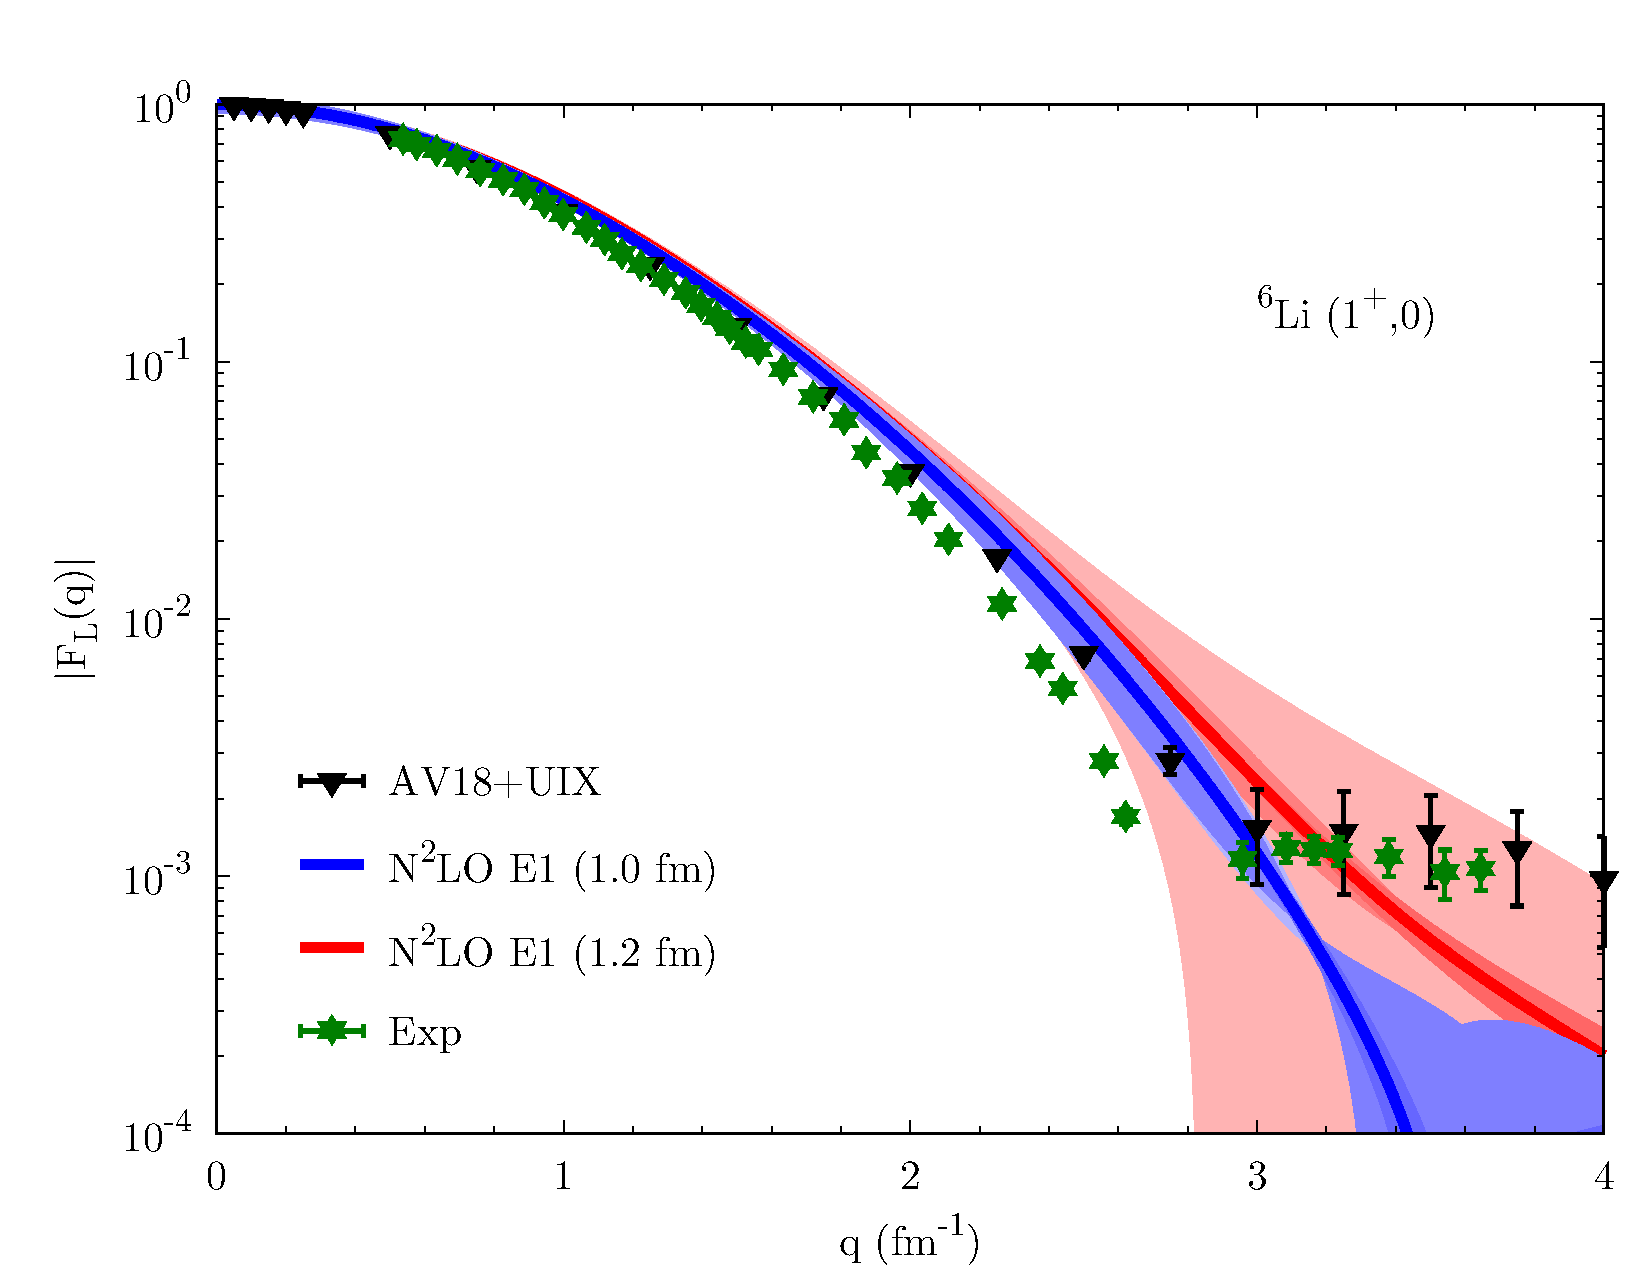
\includegraphics[width=\linewidth]{ff_li6_e1.pdf}
\caption[]{Charge form factor in \isotope[6]{Li}. The solid blue(red) line is the AFDMC result for the
N$^2$LO $E\mathbbm1$ potential with cutoff $R_0=1.0(1.2)\,\rm fm$.
Lighter shaded areas indicate the uncertainties from the truncation of the chiral expansion.
Darker shaded areas are the theoretical error bands only taking into account NLO and N$^2$LO results. 
Black triangles are the VMC one-body results for AV18+UIX~\cite{Wiringa:1998}.
The experimental data are taken from Ref.~\cite{Li:1971}.}
\label{fig:ff_li6}
\end{figure}

\begin{figure}[htb]
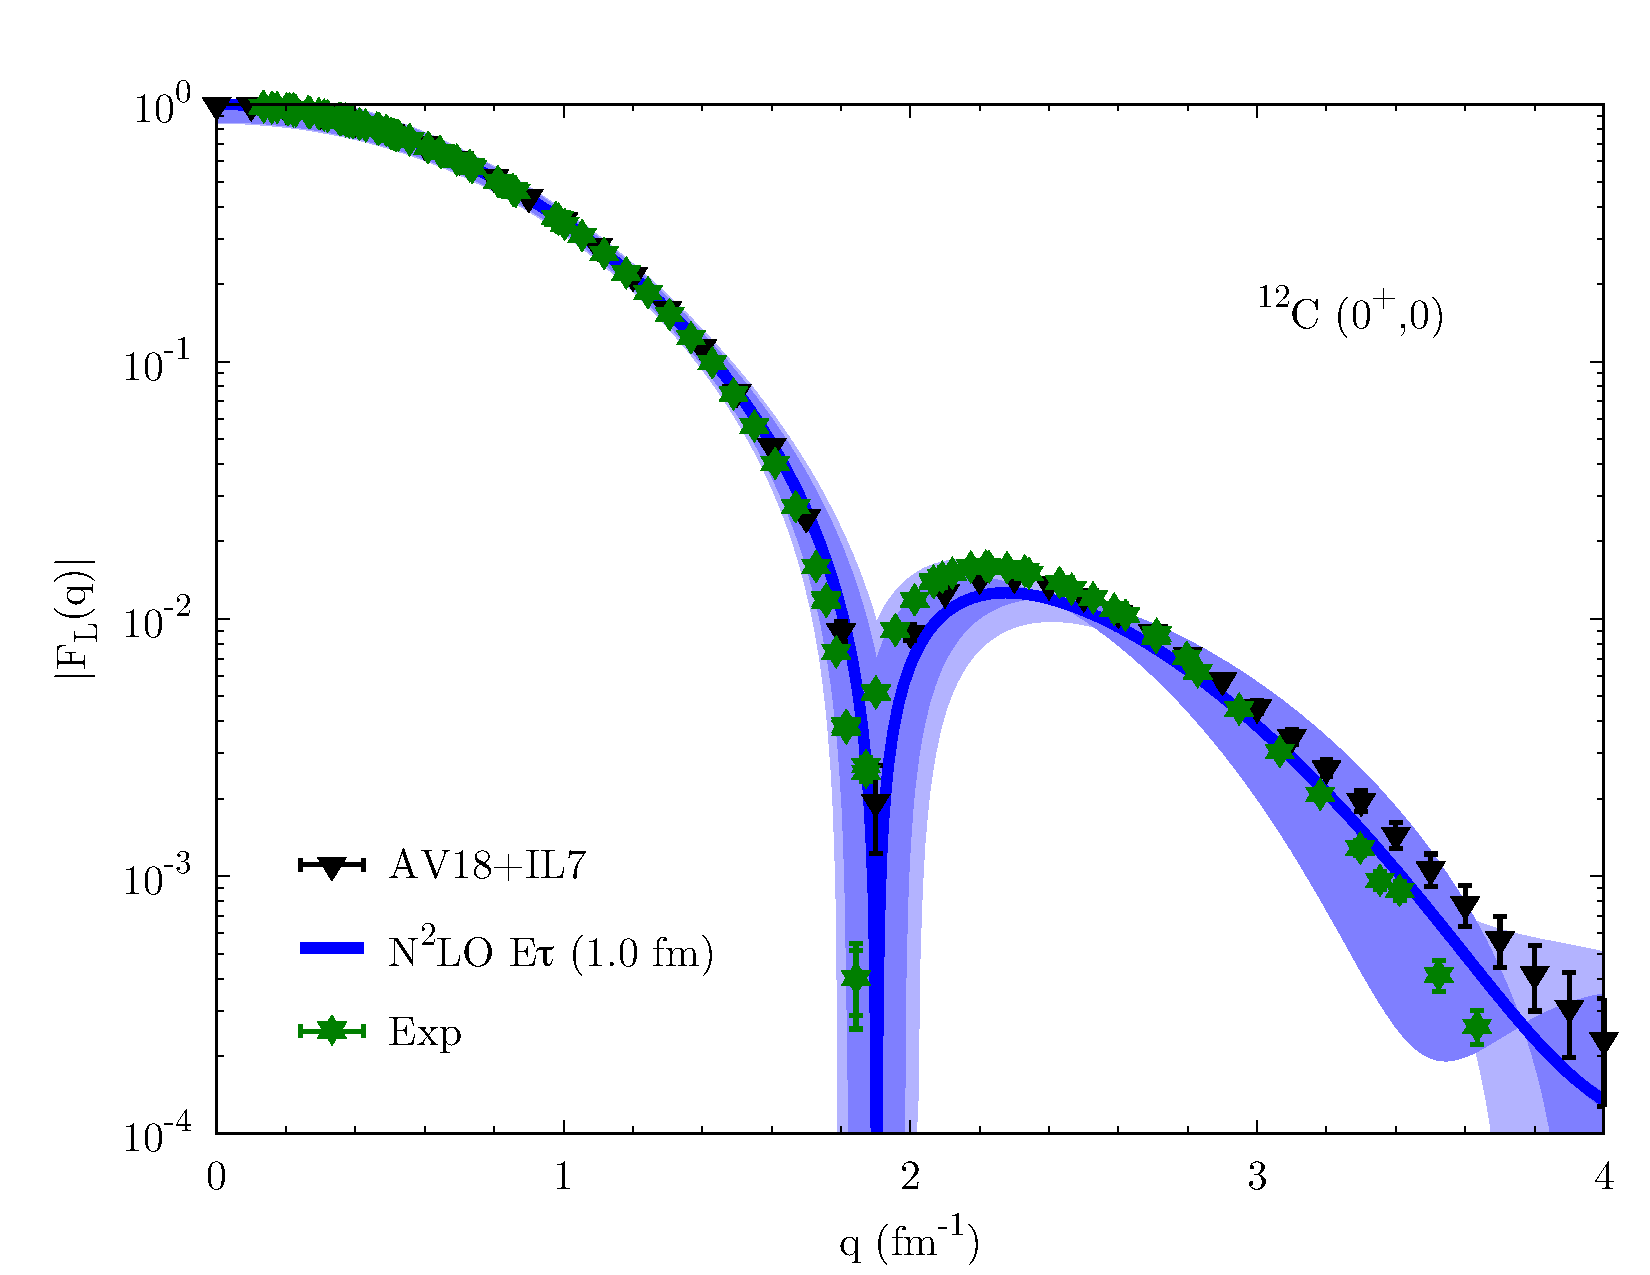
\includegraphics[width=\linewidth]{ff_c12_et.pdf}
\caption[]{Charge form factor in \isotope[12]{C}. 
In blue the AFDMC results for the $E\tau$ parametrization of the three-body
force and cutoff $R_0=1.0\,\rm fm$.
Black triangles are the GFMC one-body results for AV18+IL7~\cite{Lovato:2013}.
The experimental data are taken from Ref.~\cite{Devries:1987}.
Updated from Ref.~\cite{Lonardoni:2017afdmc}.}
\label{fig:ff_c12}
\end{figure}

\begin{figure}[htb]
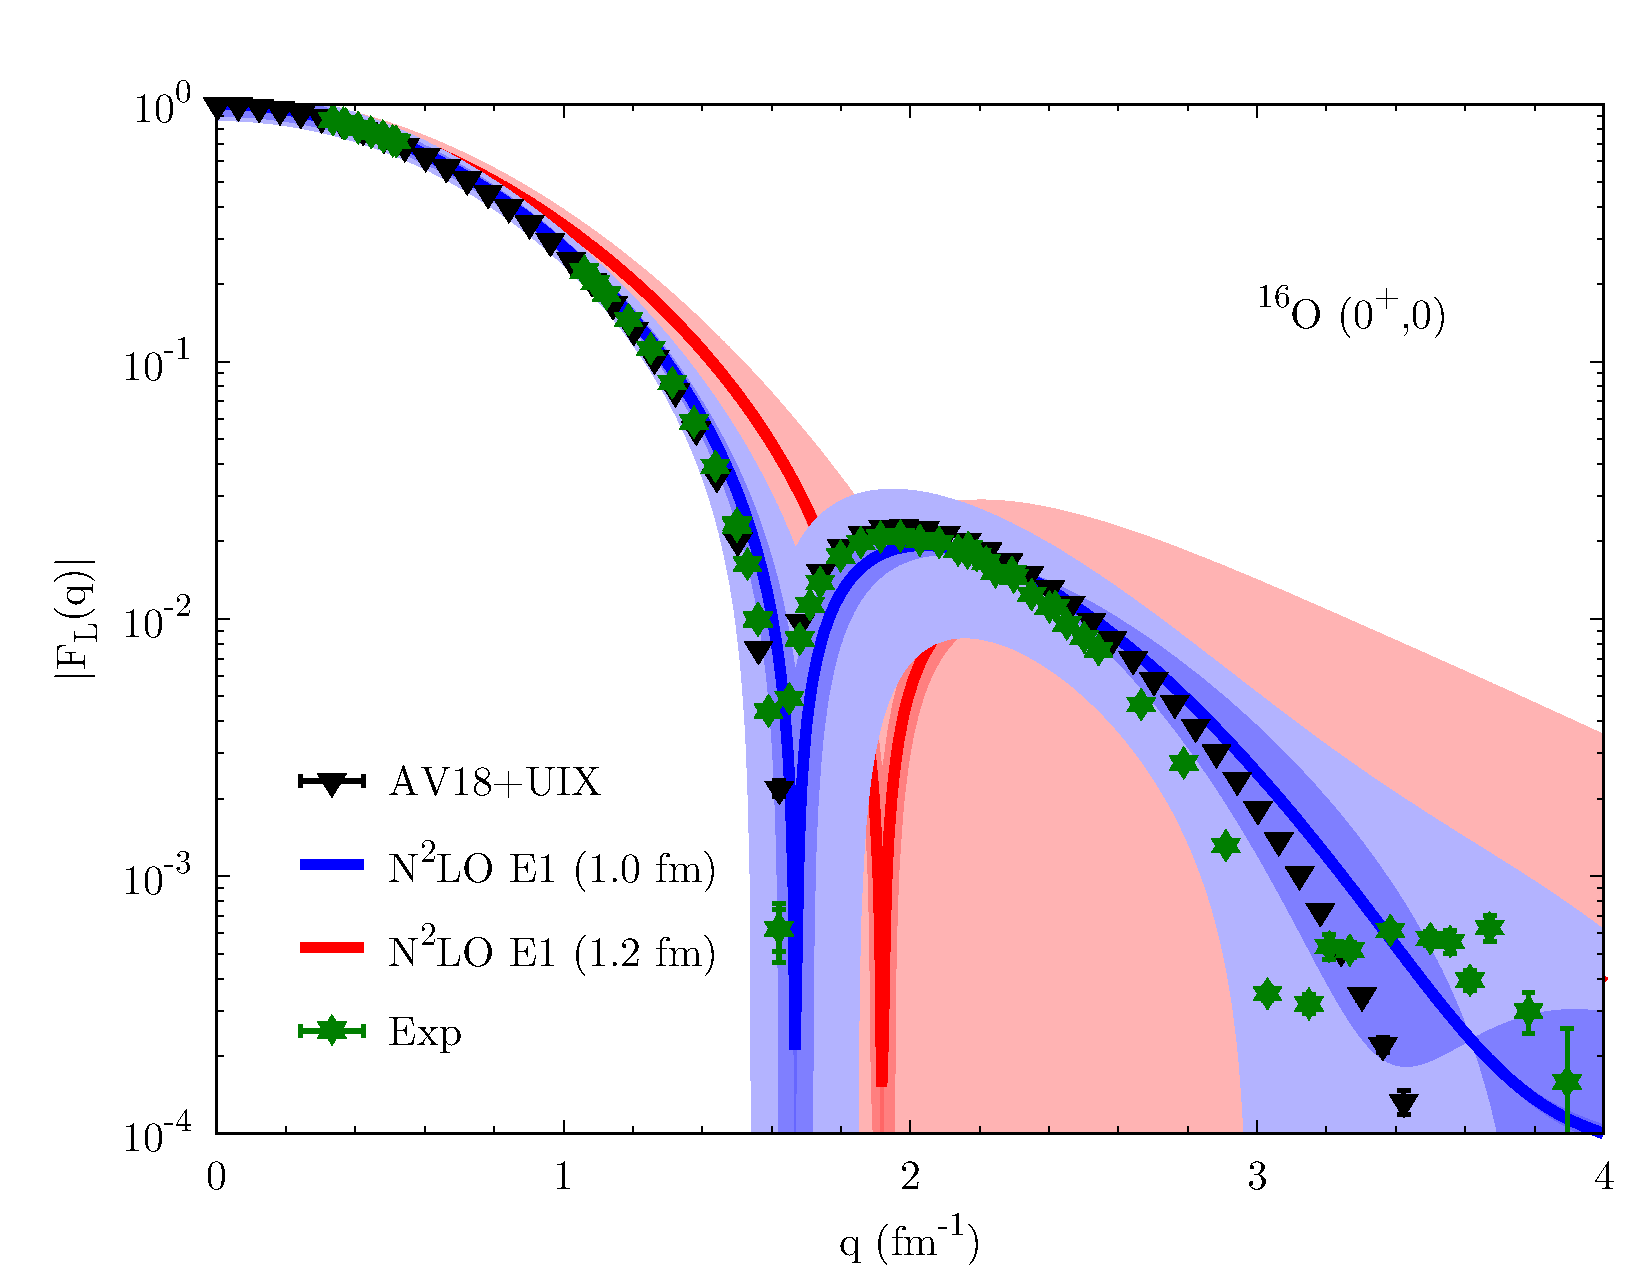
\includegraphics[width=\linewidth]{ff_o16_e1.pdf}
\caption[]{Charge form factor in \isotope[16]{O}.
In blue(red) the AFDMC results as in~\cref{fig:ff_li6}.
Black triangles are the cluster-VMC one-body results for AV18+UIX~\cite{Lonardoni:2017cvmc}.
Experimental data are from I. Sick, based on Refs.~\cite{Sick:1970,Schuetz:1975,Sick:1975}.
Updated from Ref.~\cite{Lonardoni:2017afdmc}.}
\label{fig:ff_o16}
\end{figure}

The charge form factor of \isotope[6]{Li} for the hard chiral interaction is compatible
with experimental data at low momentum. The discrepancy for $q\gtrsim2\,\rm fm^{-1}$ is most likely
due to the missing two-body currents. Similar physical picture is given for \isotope[12]{C} and
\isotope[16]{O}, for which the position of the first diffraction peak in the form factor 
is well reproduced within the band given by statistical plus theoretical uncertainties, 
and deviations from the experimental data occur at high momentum only.
For the soft chiral interaction instead, the description of the charge form factor is less 
accurate, particularly for \isotope[16]{O}, for which the position of the first diffraction 
peak is overestimated, and the slope of $F_L(q)$ for $q=0$ is underestimated, 
as reflected by the smaller charge radius compared to the experimental value.
The full truncation error estimate is provided for all the three nuclei (light bands). 
The difference between lighter and darker areas is determined by LO contributions 
to the theoretical error estimate, that are particularly important for the soft cutoff.
Finally, it is interesting to note that for all three systems, the local chiral interaction with 
cutoff $R_0=1.0\,\rm$ fm gives the same physical description of the charge form factor as 
the phenomenological potentials when only one-body charge operators are included.

Two-body densities are related to the Coulomb sum rule, that is defined as the energy integral 
of the electromagnetic longitudinal response function. As the charge form factor, the Coulomb sum rule
can be written as a ground state expectation value~\cite{Mcvoy:1962}, leading to the relation:
\begin{align}
	S_L(q)&=\frac{1}{Z} \frac{1}{G_E^{p\,2}(Q_{\rm qe}^2)}\frac{1}{1+Q_{\rm qe}^2/(4 m_N^2)} \nonumber \\
    & \times\Big\{ G_E^{p\,2}(Q_{\rm qe}^2)\,\Big[\tilde{\rho}_{pp}(q)+Z\Big] \nonumber \\
    &        +G_E^{n\,2}(Q_{\rm qe}^2)\,\Big[\tilde{\rho}_{nn}(q)+(A-Z)\Big] \nonumber \\
    &        +2\,G_E^p(Q_{\rm qe}^2)\,G_E^n(Q_{\rm qe}^2)\,\tilde{\rho}_{np}(q) \nonumber \\ 
    & -\Big[G_E^p(Q_{\rm qe}^2)\,\tilde{\rho}_p(q)+G_E^n(Q_{\rm qe}^2)\,\tilde{\rho}_n(q)\Big]^2 \Big\}, 
	\label{eq:sl}
\end{align}
where $\tilde{\rho}_{\rm{NN}}(q)$ is the Fourier transform of the two-body point-nucleon densities defined in \cref{eq:rho_NN},
and $Q^2_{\rm qe}=\vb{q}^2-\omega^2_{\rm qe}$, with $\omega_{\rm qe}$ the energy transfer 
corresponding to the quasielastic peak.
Although the Coulomb sum rule is not directly an experimental observable (experimental information can be however
extracted from the longitudinal response function, as done in Ref.~\cite{Lovato:2016} for \isotope[12]{C}), it is
still an interesting observable for the study of integral properties of the response of a nuclear many-body system to an
external probe.

We report in~\cref{fig:sl10} the Coulomb sum rule for $4\le A\le16$ using the N$^2$LO potential
with cutoff $R_0=1.0\,\rm fm$. The GFMC results for \isotope[4]{He} 
and \isotope[12]{C}~\cite{Lovato:2013,Lonardoni:2017cvmc} employing the AV18+IL7 potential are also shown for comparison.
The discrepancy between AFDMC and GFMC above $\approx 3\,\rm fm^{-1}$ is most likely due
to the missing two-body currents in the present calculation. For lower momenta the description of the sum rule 
is remarkably consistent with that provided by phenomenological potentials. 
Moreover, the results for \isotope[12]{C} are 
compatible with the available experimental data as extracted in Ref.~\cite{Lovato:2016}, 
as shown already in~\cite{Lonardoni:2017afdmc}. 
All $p$-shell nuclei show a similar profile for $S_L(q)$, with a peak around 
$1.6\,\rm fm^{-1}$ slightly more pronounced for open-shell systems $(A=6,12)$.
The same observations hold for the soft interaction, with the Coulomb sum rule 
of \isotope[4]{He} and \isotope[6]{Li} very close to those computed with 
the hard potential. Exception is the case of \isotope[16]{O}, for which $S_L(q)$
is largely different for the two cutoffs, consistently with the results for the
charge form factor, as already shown in Ref.~\cite{Lonardoni:2017afdmc}.

\begin{figure}[htb]
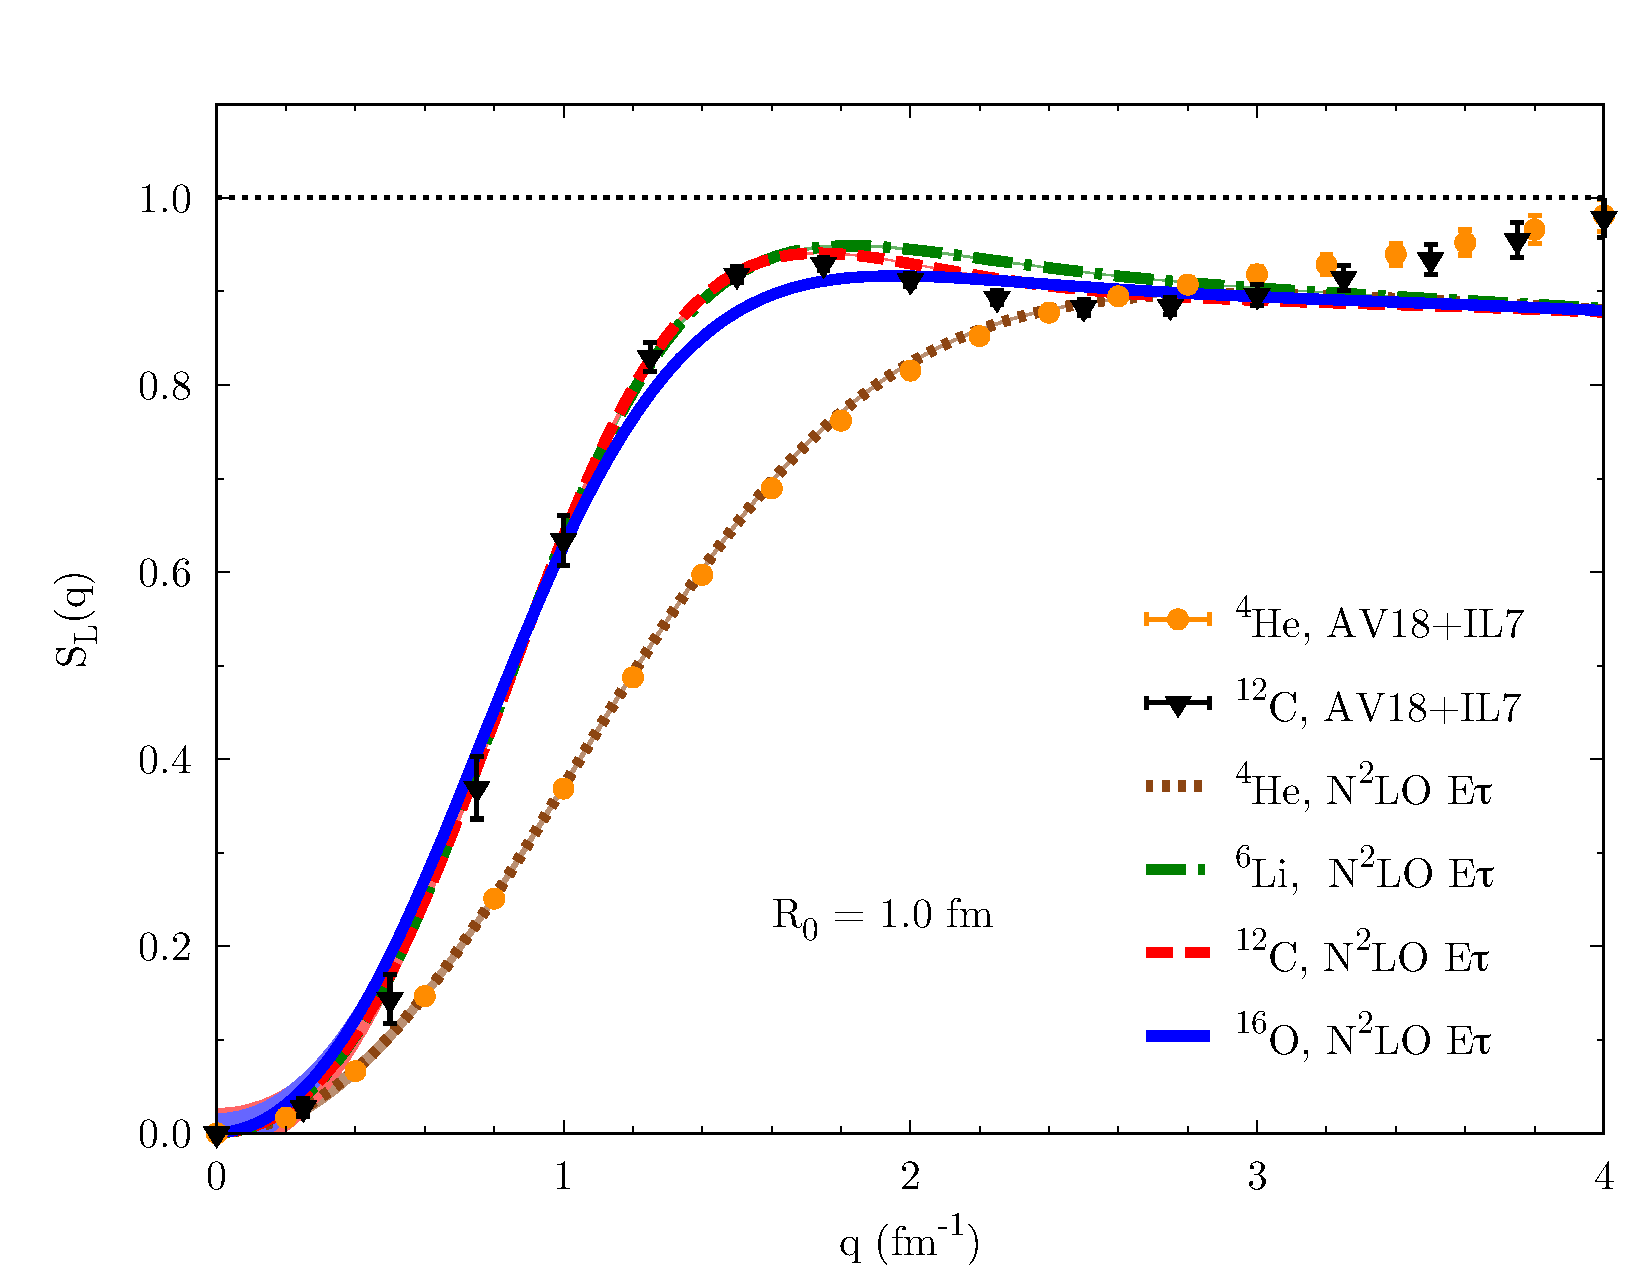
\includegraphics[width=\linewidth]{sl.pdf}
\caption[]{Coulomb sum rule for $4\le A\le16$.
Lines refer to AFDMC results for the N$^2$LO $E\tau$ potential with cutoff $R_0=1.0\,\rm fm$.
Solid symbols are the GFMC one- plus two-body results for AV18+IL7~\cite{Lovato:2013,Lonardoni:2017cvmc}. 
Shaded areas indicate the statistical Monte Carlo uncertainty.}
\label{fig:sl10}
\end{figure}


\section{Summary}
\label{sec:summ}

\red{The N$^2$LO potential for $R_0=1.0\,\rm fm$ give a good physical description 
of nuclei up to \isotope[16]{O}, consistent with experimental data and compatible 
with that of phenomenological potentials.
Softer interactions: discussion to be completed}


\acknowledgments{We thank I.~Tews, A.~Lovato, R.~F.~Garcia Ruiz
\red{ADD OTHERS} for many valuable discussions. 
The work of D.L. was was supported by the U.S. Department of Energy, 
Office of Science, Office of Nuclear Physics, under the FRIB Theory 
Alliance Grant Contract No. DE-SC0013617 titled ``FRIB Theory Center 
- A path for the science at FRIB'', and by the NUCLEI SciDAC program.
The work of S.G. and J.C. was supported by the NUCLEI SciDAC program,
by the U.S. Department of Energy, Office of Science, Office of Nuclear
Physics, under contract No. DE-AC52-06NA25396, and by the LDRD program
at LANL.
K.S. was supported by the National Science Foundation grant
PHY-1404405.
The work of J.L and A.S. was supported by the ERC Grant No.~307986
STRONGINT and the BMBF under Contract No.~05P15RDFN1.
\red{ADD OTHERS}
Computational resources have been provided by Los Alamos Open
Supercomputing via the Institutional Computing (IC) program, and by the
National Energy Research Scientific Computing Center (NERSC), which is
supported by the U.S. Department of Energy, Office of Science, under
contract DE-AC02-05CH11231 \red{ADD OTHERS}}

\appendix

\section{Calculating two-body correlations}
Given $R=\{\vb{r}_1,\dots,\vb{r}_A\}$ the particle coordinates, 
$S=\{s_1,\dots,s_A\}$ the spin/isospin configurations, 
and $|\chi_\gamma\rangle$ the $|p\uparrow\rangle$, $|p\downarrow\rangle$,
$|n\uparrow\rangle$, $|n\downarrow\rangle$ basis:
\begin{align}
	|\chi_1\rangle=|(1,0,0,0)\rangle , \nonumber \\
	|\chi_2\rangle=|(0,1,0,0)\rangle , \nonumber \\
	|\chi_3\rangle=|(0,0,1,0)\rangle , \nonumber \\
	|\chi_4\rangle=|(0,0,0,1)\rangle ,
\end{align}
let's define the Slater matrix element
\begin{align}
   S_{\alpha i}=\langle\alpha|\mathbf{r}_i\,s_i\rangle=\sum_{\gamma=1}^4\langle\alpha|\mathbf{r}_i\,\chi_\gamma\rangle\langle\chi_\gamma|s_i\rangle ,
\end{align}
where $|\alpha\rangle$ contains the radial orbitals and spherical harmonics of~\cref{eq:phi}. 
When acting with two-body correlations on the mean field part of the wave function, 
the Slater matrix is updated by each of the correlation operators. 
These updates are computed using the identity 
\begin{align}
	\det\left(S^{-1}S'\right) = \frac{\det S'}{\det S} ,
	\label{eq:invers}
\end{align}
where $S'$ is the matrix that has been updated by the action of a single operator. 
To reduce the number of operations, the ratio of determinants for a pair of operators, 
$\mathcal{O}_{ij}=\mathcal{O}_i\mathcal{O}_j$, is written in the form
\begin{align}
   \frac{\langle \Phi|\mathcal O_{ij}|RS\rangle }{\langle\Phi|RS\rangle} = \sum_{\gamma=1}^4\sum_{\delta=1}^4 d_{2b}(\chi_\gamma,\chi_\delta,ij)\langle \chi_\gamma\chi_\delta|\mathcal O_{ij}|s_is_j\rangle ,
	\label{eq:ratio}
\end{align}
with
\begin{widetext}
\begin{align}
 d_{2b}(\chi_\gamma,\chi_\delta,ij)=\frac{\langle\Phi|R,s_1,\ldots,s_{i-1},\chi_\gamma,s_{i+1},\ldots,s_{j-1},\chi_\delta,s_{j+1},\ldots,s_A\rangle}{\langle \Phi|RS\rangle} ,
\end{align}
\end{widetext}
where $\chi_\gamma$ and $\chi_\delta$ replace $s_i$ and $s_j$, respectively.
The $d_{2b}$ matrix elements are derived from the pre-calculated matrix elements $P_{\chi,ij}$
\begin{align}
   d_{2b}(\chi_\gamma,\chi_\delta,ij)=\det\begin{pmatrix}P_{\chi_\gamma,ii} & P_{\chi_\gamma,ij} \\ P_{\chi_\delta,ji} & P_{\chi_\delta,jj}\end{pmatrix} ,
\end{align}
where
\begin{align}
   P_{\chi_\gamma,ij} &=\sum_\alpha S^{-1}_{j\alpha}S_{\alpha i}(s_i\leftarrow \chi_\gamma) , \nonumber \\
   P_{\chi_\delta,ij} &=\sum_\alpha S^{\prime\;-1}_{j\alpha}S^\prime_{\alpha i}(s_j\leftarrow \chi_\delta) .
\end{align}

Though the above relations only address two-body operators, 
this method can be generalized to arbitrary $N$-body operators as well. 
To include additional operators the matrix elements $P_{\chi,ij}$ need to be updated
\begin{align}
   P_{\chi_\eta,mn}=\sum_\alpha S^{\prime\prime\;-1}_{n\alpha}S^{\prime\prime}_{\alpha m}(s_m\leftarrow \chi_\eta) ,
\end{align}
where
\begin{align}
   S^{\prime\prime}_{\alpha m}(s_m) = \left\{
   \begin{array}{cc}
      S_{\alpha m} & m \ne i\\
      \langle\alpha|\mathcal O_i|\mathbf{r}_i\,s_i\rangle  & m = i
   \end{array} .
   \right.
\end{align}
To calculate the updated inverse matrix the identity~(\ref{eq:invers}) 
is used with $S^\prime\leftarrow S^{\prime\prime}$. 
Both sides of the identity are expanded, and like terms are grouped 
noting that when $j \ne i$, $S^{\prime\prime}_{mi}=S^\prime_{mi}$.

The wave function with linear correlations (\cref{eq:psi}) is calculated 
by first acting on the coordinate and spin/isospin configurations with 
each possible operator, and calculating the sum of each term 
$\sum_{\chi_\gamma,\chi_\delta}d_{2b}(\chi_\gamma,\chi_\delta,ij)\langle\chi_\gamma,\chi_\delta|f_{ij}^p\mathcal{O}_{ij}^p|s_i s_j\rangle$. 
The expectation value of the potential on the linear wave function 
is calculated including correlation and potential operators, 
$\mathcal{O}^c_{ij}$ and $\mathcal{O}^p_{ij}$ respectively, 
organized in the form $(\mathbbm1+\mathcal{O}^c_{ij})\mathcal{O}^p_{kl}$,
that includes four potentially distinct operators. 
For this calculation the $P$ matrix is updated twice, 
once for $\mathcal{O}^c_i$ and once for $\mathcal{O}^c_j$, 
where $\mathcal{O}^c_{ij}=\mathcal{O}^c_i\mathcal{O}^c_j$ as before.  
The ratio of determinants is calculated following~\cref{eq:ratio},
using the updated distribution $d^{\prime\prime}_{2b}$.

The quadratic wave function includes the same correlation terms 
of the linear wave function plus a piece with two additional operators,
resulting in structures like $\mathbbm1+\mathcal{O}^c_{ij}+\mathcal{O}^c_{ij}\mathcal{O}^c_{kl}$. 
The operators up to linear terms are treated as above. 
The quadratic product of operators is handled in the same fashion 
as the expectation value of the potential acting on the linear wave function, i.e., 
the $P$ matrix is updated twice, once for $\mathcal{O}^c_i$ and once 
for $\mathcal{O}^c_j$, and the ratio of determinants is calculated with 
the updated distributions. It follows that the calculation of the correlation 
operators for the quadratic wave function requires $o(A^4)$ operations, compared
to $o(A^2)$ for the linear wave function.

The expectation value of the potential acting on the quadratic wave function 
requires the product of six operators $\mathcal{O}^c_{ij}\mathcal{O}^c_{kl}\mathcal{O}^p_{mn}$. 
As a result, a total of four updates are needed to calculate the quadratically correlated 
terms for the potential. After including the updated 
distributions for the $\mathcal{O}^c_{ij}$ operators, the same distributions are updated 
two more times for the $\mathcal{O}^c_{kl}$ terms. These quadratically updated distributions 
are then used to calculate the expectation value of the potential as before. 
It follows that the calculation of the expectation value of the potential acting 
on the quadratic wave function requires $o(A^6)$ operations, compared
to $o(A^4)$ for the linear wave function.

The two-body correlations of~\cref{eq:psi} have the same operator structure of the 
AV6$^\prime$ potential. The cartesian breakup of such structure generates 39 $\mathcal O^c_{ij}$ operators,  
$9\;\sigma_{\alpha i}\,\sigma_{\beta j}$, $3\;\tau_{\gamma i}\,\tau_{\gamma j}$,
and $27\;\sigma_{\alpha i}\,\sigma_{\beta j}\,\tau_{\gamma i}\,\tau_{\gamma j}$ operators. 
The number of operators can be reduced to 15 if, instead of cartesian coordinates, 
one uses the pair distance $\vb{r}_{ij}$ and two orthogonal coordinates. 
This reduces the number of operators used in the spatially dependent part of the tensor term, $3\,\bm\sigma_i\cdot\hat{\vb{r}}_{ij}\,\bm\sigma_j\cdot\hat{\vb{r}}_{ij}$, from 9 to 3.



\bibliography{biblio}
\end{document}
